\documentclass[letterpaper]{erdc}
\usepackage[all]{draftcopy}
\usepackage{amssymb}
\usepackage{amsmath}
\usepackage{amsthm}
\usepackage{calc}
\usepackage{verbatim}
\usepackage{appendix}
\usepackage{multirow}
\usepackage[subnum]{cases} % force all numcases to be subnumcases
\usepackage[section]{placeins}

\usepackage{hyperref}

\usepackage{subfig}


\graphicspath{{graphics/}{graphics/2dbox_pngs/},{graphics/saltdome_pngs/}{graphics/elder_pngs/}{graphics/saltpool3d_pngs/}{graphics/3dbox_pngs/}{graphics/henry2d_pngs/},{graphics/goswami_clement_pngs/}}

%%%%%%%%%%%%%%%%%%%%%%%%%%%%%%%%%%%%%%%%%%%%%%%%%%%%%%%%%%%%%%%%%%%%%%%%
%begin macros section from qfrkdg-macros
%%%%%%%%%%%%%%%%%%%%%%%%%%%%%%%%%%%%%%%%%%%%%%%%%%%%%%%%%%%%%%%%%%%%%%%%
%... cek macros ...

%% Create shortcut commands for various fonts and common symbols

%boldface in math mode
\newcommand{\bm}[1]{\mbox{{\boldmath ${#1}$}}}
\newcommand{\C}{\mathbb{C}}
\newcommand{\Du}{\underline{D}}
\newcommand{\del}{\nabla }
\newcommand{\deld}{\nabla \cdot}
\newcommand{\veps}{\varepsilon}
\newcommand{\eps}{\epsilon}
\newcommand{\f}{\textbf{f}}
\newcommand{\fb}{\textbf{f}}
\newcommand{\F}{\mathbb{F}}
\newcommand{\Fb}{\textbf{F}}
\newcommand{\gb}{\textbf{g}}
\newcommand{\grad}{\nabla}
\newcommand{\h}{\textbf{h}}
\newcommand{\kb}{\textbf{k}}
\newcommand{\lap}{\Delta}
\newcommand{\M}{\mathcal{M}}
\newcommand{\N}{\mathbb{N}}
\newcommand{\Norm}{\textbf{N}}
\newcommand{\n}{\textbf{n}}
\newcommand{\vp}{\varphi}
\newcommand{\vph}{\hat{\varphi}}
\newcommand{\p}{\phi}
% note:  \P is already defined to be the paragraph symbol
\newcommand{\Proj}{\mathbb{P}}
\newcommand{\Pcal}{\mathcal{P}}
\newcommand{\Q}{\mathbb{Q}}
\newcommand{\R}{\mathbb{R}}
\newcommand{\rb}{\textbf{r}}
\newcommand{\s}[1]{\mathcal{#1}}
\newcommand{\supp}{\text{supp}}
\newcommand{\Surf}{\textbf{S}}
\newcommand{\tpsi}{\tilde{\psi}}
\newcommand{\ub}{\textbf{u}}
\newcommand{\U}{\textbf{U}}
\newcommand{\vb}{\textbf{v}}
\newcommand{\V}{\mathbb{V}}
\newcommand{\wb}{\textbf{w}}
\newcommand{\x}{\textbf{x}}
\newcommand{\xh}{\hat{x}}
\newcommand{\X}{\textbf{X}}
\newcommand{\y}{\textbf{y}}
\newcommand{\yh}{\hat{y}}
\newcommand{\Y}{\textbf{Y}}
\newcommand{\Z}{\mathbb{Z}}


% vectors and tensors
\renewcommand{\vec}[1]{{\bf #1}}
\newcommand{\gvec}[1]{\mbox{{\boldmath ${#1}$}}}
\newcommand{\ten}[1]{\bar{\bm{#1}}}
%derivatives
\newcommand{\od}[2]{\frac{d {#1}}{d {#2}}}
\newcommand{\ods}[2]{\frac{d^2{#1}}{d {{#2}^2}}}
\newcommand{\pd}[2]{\frac{\partial {#1}}{\partial {#2}}}
\newcommand{\pds}[2]{\frac{\partial^2{#1}}{\partial {{#2}^2}}}
\newcommand{\pdsm}[3]{\frac{\partial^2{#1}}{\partial {#2}\,\partial {#3}}}
%funtional analysis
\newcommand{\iprod}[2]{\left( #1, #2 \right)}
\newcommand{\dprod}[2]{\left\langle #1, #2 \right\rangle}
% %real numbers
% \newcommand{\field}[1]{\mathbb{#1}}
% \newcommand{\R}{\field{R}}


%% Declare custom math operators
\DeclareMathOperator{\sech}{sech}
\DeclareMathOperator{\atanh}{atanh}
\DeclareMathOperator{\sign}{sign}
\DeclareMathOperator{\tr}{Trace}
\DeclareMathOperator{\gradsymm}{\nabla_{s}}
\DeclareMathOperator{\divergence}{div}
\DeclareMathOperator{\diag}{diag}
\DeclareMathOperator*{\argmin}{argmin}
\DeclareMathOperator*{\argmax}{argmax}
\DeclareMathOperator{\Span}{Span}
\DeclareMathOperator{\rank}{rank}


%% Sets and systems
\newcommand{\br}[1]{\left\langle #1 \right\rangle}
\newcommand{\paren}[1]{\left(#1\right)}
\newcommand{\sq}[1]{\left[#1\right]}
\newcommand{\set}[1]{\left\{\: #1 \:\right\}}
\newcommand{\setp}[2]{\left\{\, #1\: \middle|\: #2 \, \right\}}
\newcommand{\abs}[1]{\left| #1 \right|}
\newcommand{\norm}[1]{\left\| #1 \right\|}
\newcommand{\system}[1]{\left\{ \begin{array}{rl} #1 \end{array} \right.}

\newcommand{\pf}[2]{\frac{\partial #1}{\partial #2}}
\newcommand{\ipt}[2]{\langle #1,#2 \rangle}
\newcommand{\ip}{\int_{-\infty}^{+\infty}}

\renewcommand{\ker}[1]{\mathcal{N}(#1)}
\newcommand{\ran}[1]{\mathcal{R}(#1)}


%.....variable of integration 
\newcommand{\dx}{\, \mathrm{d}x} 
\newcommand{\dy}{\, \mathrm{d}y} 
\newcommand{\dz}{\, \mathrm{d}z} 
\newcommand{\dA}{\, \mathrm{d}A} 
\newcommand{\da}{\, \mathrm{d}a} 
\newcommand{\dV}{\, \mathrm{d}V} 
\newcommand{\dv}{\, \mathrm{d}v} 
\newcommand{\dt}{\, \mathrm{d}t} 
\newcommand{\ds}{\, \mathrm{d}s}
\newcommand{\dtau}{\, \mathrm{d}\tau}
\newcommand{\Th}{\mathcal{T}_\Delta}
\newcommand{\wt}{\tilde{w}}
\newcommand{\Wt}{\tilde{W}}
%delimiters
\newcommand{\pl}{\left(}
\newcommand{\pr}{\right)}
\newcommand{\sbl}{\left[}
\newcommand{\sbr}{\right]}
\newcommand{\dbl}{\left[\hspace{-0.05cm}\left[}
\newcommand{\dbr}{\right]\hspace{-0.05cm}\right]}
\newcommand{\cbl}{\left\{ }
\newcommand{\cbr}{\right\} }
\newcommand{\eqn}[1]{Equation \ref {eq:#1}}%mwf capitalized for chetn edits 12/11/07 
\newcommand{\Eqn}[1]{Equation \ref {eq:#1}} 
\newcommand{\eqnst}[2]{equations \ref{eq:#1} and \ref{eq:#2}} 
\newcommand{\Eqnst}[2]{Equations \ref{eq:#1} and \ref{eq:#2}} 
\newcommand{\eqns}[2]{equations \ref{eq:#1}--\ref{eq:#2}} 
\newcommand{\Eqns}[2]{Equations \ref{eq:#1}--\ref{eq:#2}}
\newcommand{\msection}[1]{ \vspace{.2in} {\noindent \bf #1}.}
\newcommand{\for}{\mbox{for}\quad}
% \newcommand{\argmin}{\mbox{argmin}}
% \newcommand{\argmax}{\mbox{argmax}}
\newcommand{\fig}[1]{figure \ref{fig:#1}} 
\newcommand{\Fig}[1]{Figure \ref{fig:#1}} 
\newcommand{\figst}[2]{figures \ref {fig:#1} and \ref {fig:#2}} 
\newcommand{\Figst}[2]{Figures \ref {fig:#1} and \ref {fig:#2}} 
\newcommand{\figs}[2]{figures \ref{fig:#1}--\ref{fig:#2}} 
\newcommand{\Figs}[2]{Figures \ref{fig:#1}--\ref{fig:#2}}
\newcommand{\tab}[1]{table \ref {tab:#1}} 
\newcommand{\Tab}[1]{Table \ref {tab:#1}} 
\newcommand{\tabst}[2]{tables \ref {tab:#1} and \ref {tab:#2}} 
\newcommand{\Tabst}[2]{Tables \ref {tab:#1} and \ref {tab:#2}} 
\newcommand{\tabs}[2]{tables \ref{tab:#1}--\ref{tab:#2}} 
\newcommand{\Tabs}[2]{Tables \ref{tab:#1}--\ref{tab:#2}}
\newtheorem{theorem}{Theorem}
%%velocity                                                                                                                                                                                                            
\newcommand{\vel}{\gvec{\sigma}}
\newenvironment{neqnarray}[1]{\begin{minipage}[t]{6.5in}  \begin{minipage}[b]{1.0in} #1 \end{minipage}  \begin{minipage}[b]{5.5in}\begin{eqnarray}}{\end{eqnarray}\end{minipage}\end{minipage}}
\newcommand{\bneqnarray}[2]{\\ \\ \fbox{\begin{neqnarray}{#1} #2 \end{neqnarray}}\\ \\ \noindent}

%element
\newcommand{\elem}{\Omega}
%element boundary (ind. of element)
%\newcommand{\face}{\partial \Omega}
\newcommand{\face}{\gamma}
%mesh nodes
\newcommand{\node}{\vec x}
%node star
\newcommand{\nodestar}[1]{\mathcal{E}({#1})}
%faces in element not on Neumann boundary
\newcommand{\dirIntFaces}[1]{\mathcal{F}_{i,d}({#1})}
%faces in element not on physical boundary
\newcommand{\intFaces}[1]{\mathcal{F}_{i}({#1})}
%nodes beloging to an element
\newcommand{\elemnodes}[1]{\mathcal{N}({#1})}
%nodes beloging to an element boundary
\newcommand{\facenodes}[1]{\mathcal{N}({#1})}
%left and right elements at a face
\newcommand{\lelem}{\Omega_{\ell}}
\newcommand{\relem}{\Omega_{r}}
%the left and right identifiers
\newcommand{\eleft}[1]{e_{\ell}({#1})}
\newcommand{\eright}[1]{e_{r}({#1})}
%local numbering on nodestars
\newcommand{\elemstar}{e^{\ast}}
\newcommand{\estarleft}[1]{e^{\ast}_{\ell}({#1})}
\newcommand{\estarright}[1]{e^{\ast}_{r}({#1})}
%left and right normals to face
\newcommand{\lnormal}{\vec{n}_{\ell}}
\newcommand{\rnormal}{\vec{n}_{r}}
%unique normal on face
\newcommand{\fnormal}{\vec{n}_{f}}
%local indeces on left and right
\newcommand{\ileft}{i_{\ell}}
\newcommand{\iright}{i_{r}}
%jump operator
%mwf orig
%\newcommand{\jump}[1]{\dbl #1 \dbr}
%\newcommand{\jump}[2][-0.075cm]{\left[\hspace{#1} \left[ #2 \right]\hspace{#1} \right]}
\newcommand{\jump}[2][\!]{\left[ #1 \left[ #2 \right]#1 \right]}
%multiscale formalism
\newcommand{\strongRes}{\mathcal{R}}
\newcommand{\Lop}{\mathcal{L}}
\newcommand{\LopStar}{\mathcal{L}^{\ast}}
\newcommand{\Ls}{\mathcal{L}_s}
\newcommand{\LsStar}{\mathcal{L}_s^{\ast}}
\newcommand{\LsStarApprox}{\mathcal{L}^{\ast}_{s,h}}
\newcommand{\LsHat}{\hat{\mathcal{L}}_s}
%richards equation stuff
\newcommand{\psk}{$p$-$s$-$k$}

%tables and display convenience
\newcommand{\tx}[1]{\times 10^{#1}}
%... any local macros necessary
%element identifier
\newcommand{\E}{\mathcal{E}}
%ref. element identifier
\newcommand{\hE}{\hat{\E}}
%ref. edge identifier
\newcommand{\he}{\hat{e}}
%triangulation
\newcommand{\Mh}{\mathcal{M}^h}
%shape function on element boundary
\newcommand{\eN}{\tilde{N}}
%d-1 reference element shape function
\newcommand{\heN}{\widehat{\tilde{N}}}
%for matrices
\newfont {\matFont}{cmssbx10 at 12 pt} 
\newcommand{\mat}[1]{\hbox  {\matFont #1}}
%reference element integration d's
\newcommand{\dxh}{\, \mathrm{d}\hat{x}\mathrm{d}\hat{y}}
\newcommand{\dsh}{\, \mathrm{d}\hat{s}}
\newcommand{\dth}{\, \mathrm{d}\hat{t}}
\newcommand{\ptab}{\hspace*{12pt}}

% Space functions
\newcommand{\wDel}{w_\Delta}
\newcommand{\delw}{\delta w}
\newcommand{\vDel}{v_\Delta}
\newcommand{\delv}{\delta v}
\newcommand{\uDel}{u_\Delta}
\newcommand{\delu}{\delta u}



\begin{document}

\frontmatter

\laboratory{Coastal and Hydraulics Laboratory}
\reportnum{ERDC/CHL TR-00-00}
\program{Military Engineering 6.2}

\title{Finite Element Methods for Variable Density Flows}

\author{S. R. Patty}
\affiliation{Department of Mathematics \\
Texas A\& M University\\
College Station, TX 77843-3368}

\author{M. W. Farthing \and C. E. Kees}
\affiliation{Coastal and Hydraulics Laboratory\\
  U.S. Army Engineer Research and Development Center\\
  3909 Halls Ferry Road\\
  Vicksburg, MS 39180-6199}

\coverart{coetr_gc_frontpage.pdf}
%
%rough bottom
%

\reporttype{Final Report}

% \distribution{Distribution authorized to U.S. Government Agencies
% only; Test and Evaluation; November 2005.  Other requests should be
% referred to U.S. Army Engineer Research and Development Center}

%\additionalinfo{Supersedes ERDC/CREL AF-01-23}

\begin{abstract}
  Add abstract
\end{abstract}

%\disclaimer{Some other disclaimer}
%\preparedfor{U.S. Army Engineer Research and Development Center\\
% 3909 Halls Ferry Road, Vicksburg, MS 39180-6199} 

\contractnum{K5318C}

%\monitoredby{U.S. Army Engineer Research and Development Center\\
%  3909 Halls Ferry Road, Vicksburg, MS 39180-6199}

%\preparedfor{}

\maketitle
\setcounter{tocdepth}{1}
\tableofcontents

\listoffiguresandtables
%\listoffigures
%
\chapter{Preface}

This report is a product of the the Reduced Order Modeling work unit of the
U.S. Army Engineer Research and Development Center (ERDC) Military Engineering
6.2 program.  The report was prepared by Mr. Spencer Patty of the Department of
Mathematics at Texas A\&M University, and by Drs. Christopher E. Kees and
Matthew W. Farthing of the Hydrologic Systems Branch.  General supervision was
provided by Dr. Hwai-Ping Cheng, Chief, Hydrologic Systems Branch, Dr. Ty
V. Wamsley, Chief, Flood and Coastal Storm Protection Division, and
Mr. Jos\'{e} E. S\'{a}nchez, Director, CHL; Ms. Pamela K. Kinnebrew was the
Technical Director.  LTC John Tucker was Acting Commander of ERDC, and
Dr. Jeffery P. Holland was the Director.

\mainmatter

\chapter{Introduction}

The goal of this work is to introduce a second order in time two phase flow incompressible Navier-Stokes solver using a fractional step splitting related to the pressure-correction projection methods described in \cite{guermond2006overview}.  The splitting we will be implementing was introduced in \cite{guermond2009splitting} and later analyzed in \cite{guermond2011error}.  We first introduce these splittings with a general variable density in Chapter~\ref{ch:vardensity_navierstokes_description} and compare the results of our implementation with the expected convergence results in Chapter~\ref{}  We then proceed to modify the algorithm to accomodate the two phase flow framework.  We describe the full model and then discuss the numerical results in Chapter~\ref{}

The algorithms are implemented in the finite element library \textit{Proteus} (\url{https://proteus.usace.army.mil/}), a Python library which uses Triangle (\url{http://www.cs.cmu.edu/~quake/triangle.html}) and Tetgen (\url{http://wias-berlin.de/software/tetgen/}) for the 2D and 3D mesh generators respectively.  It is a distributed multilevel finite element library designed for solving the various types of models that come up in water/civil engineering research for the Army Core of Engineers.






%
%
%
%
\chapter{Variable Density Incompressible Navier-Stokes Equations}\label{ch:vardensity_navierstokes_description}
We simulate the variable density incompressible Navier-Stokes system on a Lipshitz domain $\Lambda\subset \mathbb{R}^d$ (for $d=2,3$) and on a time domain $[0,T]$.
\begin{equation}\label{eqn:variabledensityNavierStokes}
  \begin{cases}
    \rho_t + \nabla\cdot\left( \rho \ub\right) = 0, & \mbox{for }\Lambda\times[0,T]\\
    \rho\left(\ub_t + \ub\cdot\nabla\ub  \right) + \nabla p - \mu\Delta \ub = \fb, &\mbox{for }\Lambda\times[0,T]\\
    \nabla\cdot \ub = 0, &\mbox{for } \Lambda\times[0,T]
  \end{cases}
\end{equation}
with initial and boundary conditions
\begin{equation}\label{eqn:variabledensityNavierStokesBCIC}
  \begin{cases}
    \rho(\x,0) = \rho_0(\x), & \left.\rho(\x,t)\right|_{\partial\Lambda^{in}} = a(\x,t)\\
    \ub(\x,0) = \ub_0(\x), & \left.\ub(\x,t)\right|_{\partial\Lambda} = b(\x,t)
  \end{cases}
\end{equation}
where the inflow boundary, $\partial\Lambda^{in} = \{ \x\in \partial\Lambda \:|\: \ub\cdot\n <0 \}$ where $\n$ is the outward unit normal vector.  Most all papers analyzing this method make the restrictive assumption that $\left.\ub(\x,t)\right|_{\partial\Lambda} = b(\x,t) = 0$, and thus $\partial\Lambda^{in}= \emptyset$.  However, we will discuss the inclusion of non-homogeneous dirichlet conditions on velocity and inflow conditions for density as well as other options such as natural or open boundary conditions on velocity in Section~\ref{sec:BoundaryConditions} as these are often desired in two phase flow type simulations.


%
%
%
\section{Preliminaries}


%
%
\subsection{Notation}
We discretize and subdivide the smooth spatial domain $\Lambda\subset \R^d$ into a regular uniform triangulation $\mathcal{T}_h$ with $h>0$ denoting the mesh size.  We likewise discretize the time domain $[0,T]$ into the sequence $\{ t^0=0, t^1, t^2, \dots, t^N = T\}$  with $\tau^k:= t^k-t^{k-1}$ as the step size.  If we are using a uniform time step, then $\tau^k = \tau^{k-1} = \tau = T/N$, but we leave the option for adaptive time stepping.  We use the standard notation $f^{k} := f(t=t^k,\x)$ to refer to a function or solution $f$ at a specific timestep.  When calculating norms of solutions, we often will want a combination of time and spatial norms,  thus we introduce the notation $\left( f \right)_{\tau}:= \{ f^k \}_{k=0}^{N}$ to refer to the seqence of solutions.  For instance, give a true velocity $\ub$ and a discrete solution $\ub_h$ solved for at the time steps $\{t^0,\dots, t^{N}\}$, we may want to compute the maximum norm in time and the $X$ norm in space, say the $L^2(\Lambda)^d$ or $H^1(\Lambda)^d$, etc.  We denote this as
\begin{equation}
  \left\| \left( \ub - \ub_h \right)_{\tau} \right\|_{\ell^{\infty}(X)} := \max_{1\leq k \leq N} \| \ub(t^{k}) - \ub_h^{k}\|_{X}
\end{equation}
or the $\ell^2$ norm in time, denoted
\begin{equation}
  \left\| \left( \ub - \ub_h \right)_{\tau} \right\|^2_{\ell^{2}(X)} :=  \sum_{k=1}^{N} \tau^{k}\| \ub(t^{k}) - \ub_h^{k}\|^2_{X}.
\end{equation}

We do not distinguish notation between norms of scalar functions and of vector functions.  We denote by $X_h$ the finite element space subordinate to $\mathcal{T}_h$ for the velocity vector field.  $W_h$ will be the space for density and $M_h$ the space for pressure.  Typically we will use the Taylor-Hood space $X_h \times M_h = \left(\mathbb{P}^2\left(\mathcal{T}_h\right)\right)^d\times \mathbb{P}^1\left(\mathcal{T}_h\right)$ which satisfies the LBB inf-sup condition for velocity-pressure coupling, but any set of finite element spaces satisfying the inf-sup condition can be used.  We will also typically choose $W_h = \mathbb{P}^2\left(\mathcal{T}_h\right)$.  We likewise denote the subspace $M_h^0\subset M_h$ to be the set of functions in $M_h$ with zero mean, ie $M_h^0 := \{ f_h\in M_h \:|\: \sum_{T\in\mathcal{T}_h}\int_{T}f_h dx = 0\}$.

The algorithms described below will describe methods of finding or updating the solutions at time $t^{k+1}$
\begin{equation}(\rho^{k+1}_h, \ub^{k+1}_{h}, p^{k+1}_h) \in W_h\times\X_h\times M_h  \end{equation}
given the solutions at previous time steps.  We will use first (BDF1) and second (BDF2) order approximations of time derivatives using the Backward Difference Formula (BDF) class of approximation and refer to the various algorithms by their time order and other properties of the algorithm.

%
%
\subsection{Backward Difference Formulae}
The BDF class of derivative approximations can be described generally using the following notation: An m-th order (BDF-m) approximation of the first derivative in time  uses a linear combination of the previous m time step solutions. It is convenient to use the operator $D_{\tau,m}$ to represent the BDF-m operation of first derivative in time, mainly
\begin{equation}
 \left.\frac{\partial f}{\partial t}(t,\x)\right|_{t=t^{k+1}} =  D_{\tau,m}f^{k+1} + \mathcal{O}\left(\tau^m\right)
\end{equation}
and
\begin{equation}
  D_{\tau,m}f^{k+1} =  \frac{\beta_0}{\tau^{k+1}}f^{k+1} - \displaystyle\sum_{i=1}^{m} \frac{\beta_{i}}{\tau^{k+1}} f^{k+1-i}.
\end{equation}
When it is clear from context which order, $m$, we want to use, we will drop the $m$ from the notation and simply write $D_{\tau}f^{k+1}$ for the BDf time derivative approximation.


The first order (BDF1) approximation has $\beta_0 = \beta_1 = 1$ for uniform or adaptive time steps giving
\begin{equation}
  D_{\tau,1} f^{k+1} = \frac{f^{k+1} - f^{k}}{\tau^{k+1}}.
\end{equation}
The second order (BDF2) approximation with uniform time steps has $\beta_0 = 3/2$, $\beta_1 = 2$ and $\beta_2 = -1/2$, giving
\begin{equation}  
  D_{\tau,2} f^{k+1} = \frac{3}{2\tau}f^{k+1} - \frac{2}{\tau}f^{k} + \frac{1}{2\tau}f^{k-1}.
\end{equation}
For the second order (BDF2) adaptive time stepping, we define the ratio
\begin{equation}
  r:=\tau^{k+1}/\tau^{k}
\end{equation}
then let $\beta_0 = \frac{1+2r}{(1+r)}$, $\beta_1 = 1+r$, $\beta_2 = -\frac{r^2}{(1+r)}$ giving
\begin{equation} \label{eq:bdf2withvariabletimestep} 
  D_{\tau,2} f^{k+1} = \frac{1+2r}{(1+r)\tau^{k+1}}f^{k+1} - \frac{1+r}{\tau^{k+1}}f^{k} + \frac{r^2}{(1+r)\tau^{k+1}}f^{k-1}.
\end{equation}
It is a simple calculation to show that this adaptive algorithm reduces to the uniform version above with uniform time steps, ie $r=1$.  There are higher order BDF formulae, but we will not use them here.

The adaptive BDF1 and BDF2 algorithms have truncation errors $\mathcal{O}\left(\tau^{k+1}\right)$ or $\mathcal{O}\left(\left(\tau^{k}+\tau^{k+1} \right)\tau^{k+1} \right)$ respectively, where as the uniform algorithms are $\mathcal{O}(\tau)$ and $\mathcal{O}(\tau^{2})$ respectively.
  

%
%
%
\section{Constant Density Projection Schemes}
Before moving onto the improved models, we present the basic idea of the projection scheme as introduced by Chorin and Temam.  The key is noting the Helmholtz decomposition of square integrable functions into divergence free and curl free parts
\begin{equation}
\left[ L^2(\Lambda)\right]^d = H \oplus \nabla H^1(\Lambda)
\end{equation}
where
\begin{equation}
H = \{ \vb\in \left[ L^2(\Lambda)\right]^d \:|\: \nabla\cdot \vb = 0, \left.\vb\cdot\n \right|_{\partial\Lambda} = 0  \}.
\end{equation}

Dropping the nonlinear advection terms for ease of exposition, we solve for $(\ub^{k+1}, \ut^{k+1}, p^{k+1})$ as solution of 
\begin{equation}
\begin{cases}
  \rho\ub_t - \mu\Delta\ub + \nabla p = \rho\fb,& \Lambda\times[0,T]\\
  \nabla\cdot \ub = 0,& \Lambda\times[0,T]\\
  \left.\ub\right|_{\partial\Lambda} = 0,\hspace{2mm} \left.\ub\right|_{t=0} = \ub_0,& \Lambda
\end{cases}
\end{equation}
in the following manner:
\begin{description}
  \item[Step 1] Viscous Prediction:  Find $\ut^{k+1}$ that satisfies
  \begin{equation}
    \frac{\rho}{\tau}\left(\ut^{k+1} - \ub^{k} \right) - \mu \Delta \ut^{k+1} = \rho\fb^{k+1},  \hspace{2mm} \left.\ut^{k+1}\right|_{\partial\Lambda} = 0.
  \end{equation}
  
  \item[Step 2] Projection:  Find $\ub^{k+1}, \psi^{k+1}$ that satisfy
  \begin{equation}
    \begin{cases}
    \frac{\rho}{\tau}\left(\ub^{k+1} - \ut^{k+1} \right) + \nabla \psi^{k+1} = 0 \\
    \nabla\cdot \ub^{k+1} = 0, \hspace{2mm} \left.\ub^{k+1}\cdot\n \right|_{\partial\Lambda} = 0
    \end{cases}
  \end{equation}
  
  \item[Step 3] Pressure Correction: Find $p^{k+1}$ that satisfies
  \begin{equation}
    p^{k+1} = \psi^{k+1}
  \end{equation} 
\end{description}

Notice that the second step is precisely the Helmholtz decomposition of $\ut^{k+1} = \ub^{k+1} + \nabla(\frac{\tau}{\rho} \psi^{k+1})$ with $\ub^{k+1}\in H$ and $\frac{\tau}{\rho}\psi^{k+1}\in H^1(\Lambda)$.  Thus $\ub^{k+1} = P_{H}\ut^{k+1}$ is the projection of our velocity $\ut^{k+1}$ onto the divergence free subspace $H$.

In practice, the method of solving this system is to algebraically eliminate the divergence free velocity $\ub^{k+1}$ and then solve the system for $(\ut^{k+1},\psi^{k+1}, p^{k+1})$.  The second step becomes find $\psi^{k+1}$ such that
\begin{equation}
  -\Delta\psi^{k+1} = -\frac{\tau}{\rho} \nabla\cdot \ut^{k+1}, \hspace{2mm} \left.\frac{\partial \psi^{k+1}}{\partial\n}\right|_{\partial\Lambda} = 0
\end{equation}
for which there are many fast Poisson solvers available. If desired, the divergence free velocity can then be backed out $\ub^{k+1} = \ut^{k+1} -\frac{\tau}{\rho} \nabla\psi^{k+1}$.


%
%
%
\section{Penalty-like Perturbation of Continuous Equations}
The standard approach to creating splittings has been to think about the splitting operator as a projection scheme where we have the two sequences of velocities $\{\ub^{k}\}$ and $\{\ut^{k}\}$ and the pressure increment $\{\psi^{k}\}$ that represent the Helmholtz decomposition of $L^{2}$ velocity fields into divergence free and curl free components
\begin{equation}\label{eqn:helmholtzdecompositionprojection}
  \ut^{k} = \ub^{k} + \frac{\tau}{\rho}\nabla \psi^{k}.
\end{equation}
 However, the method of solving this system is to apply the divergence operator to both sides and use the fact that $\nabla\cdot \ub^k = 0$ to algebraically eliminate $\ub^k$ from the system.  However when we applied the divergence operator to equation~(\ref{eqn:helmholtzdecompositionprojection}), we pulled the density through the divergence operator.   When density is variable, this is no longer possible.  The literature is full of methods to try to solve the resulting non-constantcoefficient problem that results from implementing this projection scheme with variable density,
\begin{equation}
  -\nabla\cdot\left(\frac{1}{\rho^{k+1}} \nabla\psi \right) = -\tau\nabla\cdot \ub^{k+1},  \hspace{1cm} \left.\partial_n \psi\right|_{\partial\Lambda} = 0.
\end{equation}  
This can be badly conditioned and rather more difficult to assemble and solve than the constant coefficient version.  In this form, it is also clear to see why later on we will require uniform lower bounds on our approximation of the density $\rho^{k+1}$.

An alternative approach is to look at the constant density projection scheme in terms of an $\epsilon$ perturbation of the original system. Thus the formerly stated projection part becomes a penalty-like adjustment that is easily generalized to the variable density framework.  The incremental pressure correction algorithm, an improvement on the original Chorin/Temam algorithm for constant density, can be expressed solely in terms of the non divergence free velocity $\ut^{k}$ and pressure $p^{k}$ in the form
\begin{equation}
  \begin{cases}
    \rho\left(\frac{\ut^{k+1} - \ut^{k}}{\tau} + \ut^{k}\cdot\nabla\ut^{k+1} \right) - \mu\Delta\ut^{k+1} + \nabla\left(p^{k} + \psi^{k}  \right) = \fb^{k+1}, & \left.\ut^{k}\right|_{\partial\Lambda} = 0\\
    \nabla\cdot\ut^{k+1} - \frac{\tau}{\rho}\Delta\psi^{n+1}=0, &\left.\partial_\n \psi\right|_{\partial\Lambda} = 0\\
    p^{k+1} = p^{k} + \psi^{k+1}
  \end{cases}
\end{equation}
This can be seen as a discrete version of the following system   
\begin{equation}\label{eqn:discreteperturbation}
  \begin{cases}
    \rho\left(\ub_t + \ub\cdot\nabla\ub  \right) + \nabla p -\mu\Delta\ub = \fb, & \left.\ub\right|_{\partial\Lambda} = 0\\
    \nabla\cdot\ub - \frac{\veps}{\rho}\Delta \psi = 0,& \left.\partial_\n \psi\right|_{\partial\Lambda} = 0\\
    \veps p_t = \psi
  \end{cases}
\end{equation}
where we have replaced difference quotients with time derivatives and substituted $\veps = \tau$ for the remaining $\tau$'s and recognized $p^{k} + \psi^{k} = p^{k} + \left( p^{k} - p^{k-1} \right) = 2p^{k} - p^{k-1} \approx p^{k+1}$ as a second order extrapolation of pressure to time $t^{k+1}$.

This is a second order $\mathcal{O}(\veps^2)$ perturbation of the constant density incompressible Navier-Stokes equations.  Simpler versions of this discrete system were observed by Rannacher in \cite{rannacher1992chorin} to be nothing more than penalties on the divergence of velocity in the momentum equation in a norm resembling the $H^{-1}$ norm.  Hence the term penalty-like algorithms.  As described in \cite{guermond2009splitting}, the system~$\left(\ref{eqn:discreteperturbation}\right)$ is the starting point for the algorithms described below.






%
%
%
\section{Penalty-Like Time-Splitting Algorithms for Variable Density}\label{sec:variabledensityAlgorithm}
\textbf{(Note rewrite this first paragraph to be more clear.)} The key to making the jump from the constant density schemes to the below defined variable density schemes is to think of the system of equations~$\left(\ref{eqn:discreteperturbation}\right)$ not as a projection scheme but as a penalty scheme with the penalty being applied on the divergence of velocity.  Then the pressure increment equation (the second one) can be easily modified to accommodate the variable density since instead of using the varying density in the second equation, we replace it with the constant $\veps = \chi \leq \min_{\x\in\overline{\Lambda}}\rho_0(\x)$ as in equation~$\left(\ref{eqn:pressureincrementlaplacian}\right)$.  This prevents us from having to solve a variable coefficient laplacian equation at each time step and instead we can solve a constant coefficient laplacian equation for the pressure increment $\psi$.  Once we have taken care of that equation, we proceed with all the standard approaches to discretizing the other momentum equations.  In particular, we will use a semi-implicit convection term $\ub^{k}\cdot\nabla\ub^{k+1}$ to remove the nonlinearity.  The rotational part of the scheme will modify the update of pressure with an extra term consisting of a penalty for divergence of velocity as seen in equation~$\left(\ref{eqn:rotationalpressureupdate}\right)$.  

The velocity described below is not explicitly enforced to be divergence free.  The penalty terms will push it in the right direction but we cannot guarantee that it will even be numerically divergence free, meaning that 
\begin{equation}
  \dprod{\ub_h}{\nabla\wb_h} = 0, \hspace{1cm}\forall\wb_h\in\X_h
\end{equation}
may not hold.  In the Proteus python library in which this will be implemented, it is possible to add some post processing to the velocity.  We can supplement the existing space after the fact with element-wise piecewise constant terms to get the Raviart-Thomas (RT0) element space and project the existing solution into that space while minimizing the residual between the existing velocity and the new projected velocity under various norms.    Thus the post processed velocity will be enforced to be divergence free and close in some sense to the computed velocity.  It is also possible to add in piecewise linear terms to get the Brezzi-Douglas-Marini-1 (BDM-1) element space.  These post processed velocities can be used for the conservation of mass equation and may provide a better solution of density transport.

\begin{remark}
We will not hereafter distinguish between the velocity and the post processed velocity.  The theory only pertains to the computed velocity and so by default we will only be using the computed velocity.  However, in some of the examples and results we may include the use of the various post processed velocities in our algorithm.
\end{remark}

We now introduce the algorithms and some theory on expected convergence rates.  We will include the BDF1 constant time step algorithm in Section~\ref{sec:BDF1ConstantTimeSteppingAlgorithm} as well as the modification for variable time stepping in Section~\ref{sec:BDF1VariableTimeSteppingAlgorithm}.  We will then describe the BDF2 constant time step and variable time step algorithms in Section~\ref{sec:BDF2ConstantTimeSteppingAlgorithm} and Section~\ref{sec:BDF2VariableTimeSteppingAlgorithm} respectively, along with some conjectured rates of convergence for them.  We will finish with some numerical examples and observed convergence rates in Section~\ref{sec:NumericalResults}.

%
%
%
\section{BDF1 Constant Time Stepping Algorithm}\label{sec:BDF1ConstantTimeSteppingAlgorithm}
We proceed in a three step update scheme.  First we update the density,  second the velocity, and third the pressure.  So given
\begin{equation}(\rho^{k}_h, \ub^{k}_{h}, p^{k}_h) \in W_h\times\X_h\times M_h  \end{equation}
we update to obtain
\begin{equation}(\rho^{k+1}_h, \ub^{k+1}_{h}, p^{k+1}_h) \in W_h\times\X_h\times M_h.\end{equation}

%
%
\subsection{Density Update}

We first solve the hyperbolic system with a monotone preserving scheme such as subgrid viscosity, edge stabilization or entropy viscosity using a DG or CG solver.  The equation of update is

\begin{equation}
  \frac{\rho^{k+1} - \rho^k}{\tau} + \nabla\cdot\left(\rho_h^{k+1}\ub^{k} \right) - \frac{\rho^{k+1}}{2}\nabla\cdot\ub^{k} = 0
\end{equation}
where the last term is a consistent stabilization which leads to unconditional stability of the scheme.   Our choice of hyperbolic solver scheme doesn't matter as long as it satisfies the following stability hypothesis:
\begin{equation}
  \chi \leq \displaystyle\min_{\x\in\overline{\Lambda}} \rho_h^{k+1}(\x), \hspace{2cm} \displaystyle\max_{\x\in\overline{\Lambda}} \rho_{h}^{k+1}(\x) \leq c_{\rho}
\end{equation}
for all $k\geq 1$.

Thus we obtain the weak solution $\rho_h^{k+1}\in W_h$ that satisfies the above requirements.  We will discuss techniques for solving the density advection equation in Section~\ref{sec:ConservationOfMassNumericalApproach}

%
%
\subsection{Velocity Update}
Once we have the density $\rho_h^{k+1}$ we can now solve for the velocity.  It turns out that we do not explicitly require this velocity to be divergence free, but simply penalize the divergence using the pressure rotational update.  We define our update terms
\begin{align*}
  \rho_h^{*} &= \frac{1}{2}\left( \rho_h^{k+1} + \rho_h^{k} \right)\\
  \delta p_h^{k} &= p_h^{k} - p_h^{k-1}\\
    p_h^{\#} &= p_h^{k} + \delta p_h^{k} = 2p_h^{k} - p_h^{k-1}
\end{align*}
so that $p_h^{\#}$ is a second order extrapolation of pressure to time $t^{k+1}$.  Next we  solve for $\ub_h^{k+1}\in\X_h$ that satisfies the following system for all $\vb_h\in\X_h$,
\begin{equation}\label{eqn:bdf1_momentum_constanttimestep}
  \begin{split}
\dprod{ \frac{\rho_h^{*}\ub_h^{k+1}-\rho_h^{k}\ub_h^{k} }{\tau} }{\vb_h} + \dprod{ \rho_h^{k+1}\ub_h^{k}\cdot\nabla\ub_h^{k+1} }{\vb_h}+ \mu\dprod{ \nabla \ub_h^{k+1} }{\nabla\vb_h}&\\
 + \dprod{ \frac{1}{2}\nabla\cdot\left(\rho_h^{k+1}\ub_h^{k}\right)\ub_h^{k+1} }{\vb_h} +\dprod{\nabla p_h^{\#}}{\vb_h} &= \dprod{\fb^{k+1}}{\vb_h}.
\end{split}
\end{equation}

We note that Equation~(\ref{eqn:bdf1_momentum_constanttimestep}) can be rewritten in a more recognizable format that emphasizes the consistent stabilizing term as a scaled version of conservation of mass, namely
\begin{equation}\label{eqn:bdf1morerecognizableform}
  \begin{split}
\dprod{\rho_h^{k} \frac{\ub_h^{k+1}-\ub_h^{k} }{\tau} }{\vb_h} &+ \dprod{ \rho_h^{k+1}\ub_h^{k}\cdot\nabla\ub_h^{k+1} }{\vb_h} + \mu\dprod{ \nabla \ub_h^{k+1} }{\nabla\vb_h}+\dprod{\nabla p_h^{\#}}{\vb_h}\\
 &+ \frac{1}{2}\dprod{ \left(\frac{\rho_h^{k+1} - \rho_h^{k}}{\tau} + \nabla\cdot\left(\rho_h^{k+1}\ub_h^{k}\right)  \right )\ub_h^{k+1} }{\vb_h} = \dprod{\fb^{k+1}}{\vb_h}.
\end{split}
\end{equation}

%
%
\subsection{Pressure Update}\label{sec:bdf1pressureupdate}
\begin{remark}
For the second order algorithm, there are two options for pressure update, the so called \textbf{standard form} and the \textbf{rotational form} which differ only in an additional term being added to the pressure update.  For the first order algorithm, we could likewise implement a rotational form but it does not improve our convergence rates so here we will only give the standard algorithm.  The second order description in Section~\ref{sec:bdf2pressureupdate} will go into more details on these two approaches.
\end{remark}

Now that we have $\rho_h^{k+1}$ and $\ub_h^{k+1}$, we solve for the pressure increment $\psi_h^{\flat}\in M_h^0$ which then allows us to solve for the pressure $p_h^{k+1}\in M_h$.  
Recalling that $\chi \leq \displaystyle\min_{\x\in\overline{\Lambda}} \rho_h^{k+1}(\x)$ (note that we will often choose it to be the minimum), we let $\psi_h^{\flat}\in M^0_h$ be the weak solution of
\begin{equation}\label{eqn:pressureincrementlaplacian}
  \Delta \psi^{\flat} = \frac{\chi}{\tau}\nabla\cdot \ub^{k+1}, \hspace{1cm} \left.\partial_\n\psi^{\flat}\right|_{\partial\Lambda} = 0
\end{equation}
with $\int_{\Lambda} \psi^{\flat} d\x = 0$.  That is, find $\psi_h^{\flat}\in M_h^0$ (functions with mean zero) such that
\begin{equation}
  \dprod{\nabla\psi_h^{\flat}}{\nabla r_h} = \frac{\chi}{\tau}\dprod{\ub_h^{k+1}}{\nabla r_h}
\end{equation}
for all $r_h \in M_h$.  If we don't build the mean zero property into the finite element space, then equation~(\ref{eqn:pressureincrementlaplacian}) is an under determined system.  It is often quite difficult to obtain basis functions with mean zero, so a common approach to solving the system with this setup is to fix the value at one degree of freedom, solve the system, calculate the mean and subtract it off of the solution.  Thereby we move the solution into the zero mean subset $M_h^0\subset M_h$. 

 Once we have the pressure correction term, $\psi^{\flat}_h\in M_h^0$, we update the pressure as
\begin{equation}\label{eqn:rotationalpressureupdate}
  p^{k+1} = \psi^{\flat} + p^{k}
\end{equation}
which can be done by simple addition instead of solving the projection scheme 
\begin{equation}
  \dprod{p_h^{k+1}}{r_h} = \dprod{\psi_h^{\flat} + p_h^{k}}{r_h}.
\end{equation}

% or in other words, we solve for $p_h^{k+1}\in M_h$ such that for all $r_h\in M_h$
% \begin{equation}
%   \dprod{p_h^{k+1}}{r_h} = \dprod{\psi_h^{\flat} + p_h^{k}}{r_h} + \mu\dprod{\ub_h^{k+1}}{\nabla r_h}.
% \end{equation}
% The last term involving the divergence of velocity makes this the \textbf{rotational form} and leaving it off is the \textbf{standard form}.  In standard form, it is simple enough to just add $p_h^{k+1}$ and $\psi_h^{\flat}$ to update $p_h^{k+1}$ instead of solving the linear system.
%

%
%
\subsection{Summary of BDF1 Constant Time Step Incremental Algorithm}\label{subsec:BDF1constantTimeSummary}
Given $(\rho^{k}, \ub^{k}, p^{k})\in W_h\times \X_h\times M_h$ where the spaces $\X_h\times M_h$ satisfy the standard LBB inf-sup conditions, 
\begin{description}
  \item[Step 1] Density Update: Solve for $\rho^{k+1}\in W_h$ such that
\begin{equation}
  \frac{\rho^{k+1} - \rho^k}{\tau} + \nabla\cdot\left(\rho_h^{k+1}\ub^{k} \right) - \frac{\rho^{k+1}}{2}\nabla\cdot\ub^{k} = 0.
\end{equation}
using a monotone preserving hyperbolic transport method.  

\item[Step 2] Viscous Prediction: Set 
\begin{equation}\label{eq:pressureextrapolation_uniformtimestep}
  p^{\sharp} = 2p_h^{k} - p_h^{k-1}
\end{equation}
and find $\ub^{k+1}_h\in\X_h$ such that for all $\vb_h\in\X_h$,
\begin{equation}
  \begin{split}
\dprod{ \rho_h^{k}\frac{\ub_h^{k+1}-\ub_h^{k} }{\tau} }{\vb_h} + \dprod{ \rho_h^{k+1}\ub_h^{k}\cdot\nabla\ub_h^{k+1} }{\vb_h} + \mu\dprod{ \nabla \ub_h^{k+1} }{\nabla\vb_h}& \\
+ \frac{1}{2}\dprod{\left[\frac{\rho^{k+1}-\rho^{k}}{\tau} + \nabla\cdot\left(\rho_h^{k+1}\ub_h^{k}\right)\right]\ub_h^{k+1} }{\vb_h} +\dprod{\nabla p_h^{\sharp}}{\vb_h} &= \dprod{\fb^{k+1}}{\vb_h}.
\end{split}
\end{equation}

\item[Step 3] Projection: Find $\psi_h^{\flat}\in M^0_h$ such that for all $r_h\in M_h$,
\begin{equation}
  \dprod{\nabla\psi_h^{\flat}}{\nabla r_h} = \frac{\chi}{\tau}\dprod{\ub_h^{k+1}}{\nabla r_h}
\end{equation}
where $\chi \leq \displaystyle\min_{\x\in\overline{\Lambda}}\rho_0(\x)$ 

\item[Step 4] Pressure Correction: Update the pressure $p_h^{k+1}\in M_h$, 
\begin{equation}
p^{k+1}_h = p^{k}_h + \psi^{\flat}_h.
\end{equation}
\end{description}
Thus we have solved for $(\rho_h^{k+1}, \ub_h^{k+1}, p_h^{k+1})$ and can move on to the next time step.

%
% %
% %
% \subsection{Error analysis of BDF1 Constant Time Step Incremental Algorithm}
% The stability of the above algorithm is proved in \cite{guermond2009splitting} and the error analysis was carried out in \cite{guermond2011error}.  We refer the reader to those articles for details and give the main results contained in Theorem 4.2 of \cite{guermond2011error}.
%
% We define the \textbf{Stokes projection}, $\left(\wb_h(t),q_h(t)\right) \in \X_h\times M_h$, of the solution $\left(\ub(t),p(t)\right)$ to (\ref{eqn:variabledensityNavierStokes})-(\ref{eqn:variabledensityNavierStokesBCIC}) to be the pair that solves
% \begin{equation}
%   \begin{cases}
%     \mu\dprod{\nabla\wb_h(t)}{\nabla\vb_h} + \dprod{\nabla q_h(t)}{\vb_h} = \mu\dprod{\nabla \ub(t)}{\nabla\vb_h} - \dprod{p(t)}{\nabla\cdot\vb_h}, & \forall \vb_h \in \X_h\\
%     \dprod{\wb_h(t)}{\nabla r_h} = 0, & \forall r_h\in M_h
%   \end{cases}
% \end{equation}
%
% \begin{theorem}
%   Assume that the true solution to (\ref{eqn:variabledensityNavierStokes}) and (\ref{eqn:variabledensityNavierStokesBCIC}) satisfies (with $l\geq 1$)
%   \begin{equation}
%     \ub\in W^{2,\infty}\left(\mathbf{H}_0^1(\Lambda)\cap \mathbf{H}^{\ell+1}(\Lambda)\right), \hspace{1cm} p\in W^{1,\infty}\left(H^{\ell}(\Lambda) \right)
%   \end{equation}
%   Let $(\ub_h)_{\tau}$ be the solutions of velocity as described in Subsection~\ref{subsec:BDF1constantTimeSummary}.  Then if one of either
%   \begin{equation}
%     \|p_h^0 - q_h^0 \|_{L^2(\Lambda)} \leq c h^{\frac{\ell+1}{2}}
%   \end{equation}
%   or
%   \begin{equation}
%     \|p_h^0\|_{H^1(\Lambda)} \leq c \hspace{0.5cm} \mbox{and} \hspace{0.5cm} \dprod{\ub_h^0}{\nabla r_h} = 0 \hspace{0.25cm} \forall r_h\in M_h
%   \end{equation}
%   is satisfied, then
%   \begin{equation}
%     \|\left(\ub - \ub_h\right)_{\tau} \|_{\ell^{\infty}(\mathbf{L}^2(\Lambda))} \leq c\left( \tau + h^{\min(\ell+1,s)} \right)
%   \end{equation}
%   and
%   \begin{equation}
%     \|\left(\ub - \ub_h\right)_{\tau} \|_{\ell^{2}(\mathbf{H}^1(\Lambda))} \leq c\left( \tau + h^{\min(\ell,s)} \right)
%   \end{equation}
% \end{theorem}
%
% \begin{remark}
%   Here $s>0$ is a constant that deals with the coupling between velocity and our solution of density transport.  In particular it depends on the method we use to solve the mass conservation.  The details are described in Section 4.2 of \cite{guermond2011error} (using the symbol $m$ instead of $s$) where they conjecture that one can obtain $s=1$ by approximating the mass conservation with a linear first-order viscosity or first-order level set or phase field approach.  They further conjecture that $s>1$ if one uses a nonlinear stabilization technique like discontinuous Galerkin with limiters or entropy viscosity.
% \end{remark}



%
%
%
\section{Hyperbolic Conservation of Mass Algorithms}\label{sec:ConservationOfMassNumericalApproach}

\textbf{ Add stuff here}



%
%
%
\section{BDF2 Constant Time Stepping Algorithm}\label{sec:BDF2ConstantTimeSteppingAlgorithm}

The above BDF1 schemes are proved in \cite{guermond2011error} to be first order accurate in time for the $\mathbf{L}^2(\Lambda)$ and $\mathbf{H}^1(\Lambda)$ norms of velocity.  However, because we have used a second order extrapolation of pressure
\begin{equation}
  p^{\sharp}_h = p_h^{k} + \delta p_h^{k} = 2p^{k}_h-p^{k-1}_h \approx p_h^{k+1} + \mathcal{O}\left(\tau^2 \right)
\end{equation}
to split the system of equations, the splitting error of the algorithm is expected to be second order.  Thus it seems logical to introduce a second order approximation to the time derivative for the velocity equations.  Likewise it might be advantageous to use a second order extrapolation of velocity 
\begin{equation}
  \ub^{*}_h = 2\ub_h^{k}  - \ub_h^{k-1}
\end{equation}
for the semi-implicit convection term, $\ub_h^{*}\cdot\nabla\ub_h^{n+1}$, again eliminating the nonlinearity and preserving the second order in time approximation.


%
%
\subsection{Density Update}
Again, the approach to solving this hyperbolic equation is not specified here but is discussed in Section~\ref{sec:ConservationOfMassNumericalApproach}.  We will choose a second order hyperbolic scheme that preserves the following stability properties.  First, that there are constants $\chi, c > 0$ such that 
\begin{equation}
  \chi \leq \displaystyle\min_{\x\in\overline{\Lambda}} \rho_h^{k+1}(\x),  \hspace{1.5cm} \displaystyle\sup_{\x\in\overline{\Lambda}}\rho_h^{k+1}(\x) \leq c \hspace{1cm} \forall k\geq 1
\end{equation}
and secondly that when solving for $\rho_h^{k+1}\in W_h$, that there is a uniform constant $M$ such that
\begin{equation}
  \displaystyle\max_{0\leq n\leq k-1} \left \| \frac{\rho_h^{n+1} - \rho_h^{n}}{\tau}\right\|_{L^{\infty}(\Lambda)} \leq M\chi.
\end{equation}

%
%
\subsection{Velocity Update}
We define
\begin{equation}
  \rho_h^{*} := \frac{3}{2}\rho_h^{k+1} - \frac{2}{3}\rho_h^{k} + \frac{1}{6}\rho_h^{k-1} = \rho_h^{k+1} + \frac{1}{6}\left(3\rho_h^{k+1} -4\rho_h^{k} + \rho_h^{k-1} \right)
\end{equation}
\begin{equation}
  p_h^{\sharp} := p_h^{k} + \frac{4}{3}\psi_h^{k} - \frac{1}{3}\psi_h^{k-1}.
\end{equation}
and the second order extrapolation of velocity
\begin{equation}\label{eq:velocityextrapolation_uniformtimestep}
  \ub^{*}_h = 2\ub_h^{k}  - \ub_h^{k-1}.
\end{equation}
Now compute $\ub_h^{k+1}\in\X_h$ so that for all $\vb_h\in\X_h$,
\begin{equation}\label{eqn:bdf2lessrecognizableform}
  \begin{split}
    \dprod{\frac{3\rho_h^{*}\ub_h^{k+1} - 4\rho_h^{k+1}\ub_h^{k} + \rho_h^{k+1}\ub_h^{k-1}}{2\tau}}{\vb_h}  + \dprod{\mu\nabla\ub_h^{k+1}}{\nabla\vb_h} &\\
   + \dprod{\nabla p_h^{\sharp}}{\vb_h} + \dprod{\rho_h^{k+1}\ub_h^{*}\cdot\nabla\ub_h^{k+1} + \frac{1}{2}\ub_h^{k+1}\nabla\cdot\left( \rho_h^{k+1}\ub_h^{*} \right)}{\vb_h} &= \dprod{\fb^{k+1}}{\vb_h}
  \end{split}
\end{equation}
Notice that we only use $\rho_h^{k+1}$ or $\rho_h^{*}$ in the above equation.

\begin{remark}
Again, as in the BDF1 case (equation~(\ref{eqn:bdf1morerecognizableform})), we can rearrange terms so that equation~(\ref{eqn:bdf2lessrecognizableform}) is a little more recognizable.  This is done in the general description in Section~\ref{sec:generalalgorithm}.
\end{remark}

\begin{remark}
If the terms are smooth enough, then we have
\begin{align}
  &\frac{3\rho_h^{*}\ub_h^{k+1}-4\rho_h^{k+1}\ub_h^{k} +\rho_h^{k+1}\ub_h^{k-1}}{2\tau} +\frac{1}{2}\nabla\cdot\left(\rho_h^{k+1}\ub_h^{*}\right)\ub_h^{k+1}\\
   &= \rho_h^{k+1}\left(\frac{3\ub_h^{k+1} - 4\ub_h^{k} + \ub_h^{k-1}}{2\tau}\right) + \frac{1}{2} \left( \frac{3\rho_h^{k+1} -4\rho_h^{k} + \rho_h^{k-1}}{2\tau} + \nabla\cdot\left(\rho_h^{k+1}\ub_h^{*}\right)\right)\ub_h^{k+1}\\
  &= \left.\left(\rho_h\frac{d\ub_h}{dt} \right)\right|_{t=t^{k+1}} + \left.\frac{1}{2} \left( \frac{d\rho_h}{dt} +\nabla\cdot\left(\rho_h\ub_h\right)\right)\right|_{t=t^{k+1}}\ub_h^{k+1} + \mathcal{O}(\tau^2)\\
  &=\left.\left(\rho_h\frac{d\ub_h}{dt} \right)\right|_{t=t^{k+1}} + \mathcal{O}(\tau^{2})
\end{align}
where we have used (a) the fact that $\ub_h^{*}$ is a second order in time approximation to $\ub_h^{k+1}$ and (b) the conservation of mass property to cancel the second term for the last step.
\end{remark}




%
%
\subsection{Penalty Term Update}
We compute the pressure correction $\psi_h^{k+1}\in M^0_h$ so that for all $r_h\in M_h$,
\begin{equation}
  \dprod{\nabla\psi_h^{k+1}}{\nabla r_h} = \frac{3\chi}{2\tau}\dprod{\ub_h^{k+1}}{\nabla r_h}.
\end{equation}

\begin{remark}
  A numerical technique for the above system for $\psi_h^{k+1}\in M_h^0$ with zero mean is described in Section~\ref{sec:bdf1pressureupdate}.
\end{remark}

%
%
\subsection{Pressure Update}\label{sec:bdf2pressureupdate}
\begin{remark}
  There are two options for how to correct the pressure.  The \textbf{standard form} which is simply the update $p_h^{k+1} = p_h^{k} + \psi_h^{k+1}$, and the \textbf{rotational form} which adds an additional term $\nabla\cdot\left(\mu\ub^{k+1}_h\right)$ to the update.  Using the rotational form increases the accuracy of pressure and the $H^1$ norm of velocity by $\tau^{1/2}$ and so is the prefered method.  It is analyzed in \cite{guermond2004error} for constant density and viscosity.
\end{remark}
Finally, we update the pressure with the pressure correction and the rotational term $\nabla\cdot\left(\mu\ub^{k+1}_h\right)$
\begin{equation}
  p_h^{k+1} = p_h^{k} + \psi_h^{k+1} - \nabla\cdot\left(\mu\ub^{k+1}_h\right)
\end{equation}
meaning we seek $p_h^{k+1}\in M_h$ such that for all $r_h\in M_h$
\begin{equation}
  \dprod{p_h^{k+1}}{r_h} = \dprod{p_h^{k} + \psi_h^{k+1}}{r_h} + \dprod{\mu\ub_h^{k+1}}{\nabla r_h}.
\end{equation}


\begin{remark}
Now that we have defined $\psi_h^{k}$, we can show what $p_h^{\sharp}$ represents.  In the non-rotational scheme, we have
\begin{equation}
  \psi_h^{k+1} = p_h^{k+1} - p_h^{k}
\end{equation}
so that
  \begin{align}
    p_h^{\sharp} &= p_h^{k} + \frac{4}{3}\psi_h^{k} - \frac{1}{3}\psi_h^{k-1}\\
    &= p_h^{k} + \frac{4}{3}\left(p_h^{k} - p_h^{k-1}\right) - \frac{1}{3}\left(p_h^{k-1} - p_h^{k-2}\right)\\
    &= \frac{7}{3}p_h^{k} - \frac{5}{3}p_h^{k-1}+ \frac{1}{3}p_h^{k-2} \\
    &= \frac{1}{3}\left( 3p_h^{k} - 3p_h^{k-1} + p_h^{k-2} \right) + \frac{2}{3}\left(2p_h^{k} - p_h^{k-1}  \right)\\
    &= \frac{1}{3}p_h^{k+1} + \mathcal{O}(\tau^{3}) + \frac{2}{3} p_h^{k+1} + \mathcal{O}(\tau^{2})\\
    &= p_h^{k+1} + \mathcal{O}\left(\tau^2+\tau^3\right)
  \end{align}
  since the following extrapolation schemes hold for smooth $g(t)$ with constant time step $\tau>0$, where $g^{k} := g\left(t^{k}\right)$, and $t^k = t^0+k\tau$:
  \begin{equation}
    g^{k+1} = 3g^k - 3g^{k-1}+g^{k-2} + \mathcal{O}(\tau^3) \mbox{ and } g^{k+1}=2g^{k} - g^{k-1}+\mathcal{O}(\tau^2).
  \end{equation}
  
  Another way of analyzing it is to recognize that 
  \begin{align}
    p^{\sharp}_h &= \frac{7}{3}p_h^{k} - \frac{5}{3}p_h^{k-1}+ \frac{1}{3}p_h^{k-2} \\
    &= 2p_h^k - p_h^{k-1} + \frac{\tau^2}{3}\left(\frac{p_h^{k} - 2p^{k-1}_h + p_h^{k-2}}{\tau^2}  \right)\\
    &= p_h^{k+1} + \mathcal{O}(\tau^{2}) + \frac{\tau^2}{3}\left( p_{tt}^{k-1} + \mathcal{O}(\tau^{2}) \right)\\
    &= p_h^{k+1} + \mathcal{O}(\tau^2)
  \end{align}
  Whatever the approach, it gives us a higher order approximation to the pressure $p_h^{k+1}$ which is consistent with the original equations.
  
  When the rotational scheme is used, there is an extra set of terms, which can be expanded in Taylor series in time 
  \begin{align}
    -\frac{4}{3}\nabla\cdot\left[\mu\ub_h^{k}\right] + \frac{1}{3}\nabla\cdot\left[\mu\ub_h^{k-1}\right] &= -\nabla\cdot\left[\mu\left(\frac{4}{3}\ub_h^{k} - \frac{1}{3}\ub_h^{k-1} \right)\right]\\
    &= -\nabla\cdot\left[\mu \left(2\ub_h^{k} - \ub_h^{k-1}  \right) + \frac{2}{3}\tau\mu\left( \frac{\ub^{k} - \ub^{k-1}}{\tau} \right)   \right]\\
    &= -\nabla\cdot\left[\mu\left( \ub^{k+1} + \frac{2}{3}\tau\ub_t^{k} + \mathcal{O}(\tau^{2}) \right)\right]\\
    &= -\nabla\cdot\left[\mu\ub^{k+1}\right] + \frac{2}{3}\tau\nabla\cdot\left[\mu\ub_t^{k}\right] + \mathcal{O}(\tau^{2})
  \end{align}
  which can be seen as a penalty term on the divergence of velocity at time $t^{k+1}$.  The first term combines with the diffusion term to fix part of the artificial boundary conditions that are imposed by this splitting and the rest is absorbed as a penalty.  More details can be found in \cite{guermond2004error} and in the appendix below.
\end{remark}

% \begin{remark}
% It turns out we can do a similar trick with the general coefficients $\beta_0$, $\beta_1$ and $\beta_2$ if we rewrite them using the ratio $r = \tau^{k+1}/\tau^{k}$, however we must use the proper scaling for variable time stepping
% \begin{equation}
%   p^{\sharp}_h = p_h^{k} + r\left(\frac{\beta_1}{\beta_0}\psi^{k} + \frac{\beta_1}{\beta_0}\psi^{k-1}  \right).
% \end{equation}
% Notice the extra factor $r$ in there similar to the extension of $2p_h^{k}-p_h^{k-1}$ to $p_h^{k} + r(p_h^k - p_h^{k-1})$.  Recalling the definitions implicit in equation~(\ref{eq:bdf2withvariabletimestep}) for the BDF2 coefficients and of the pressure increment, $\psi^{k}_h = p^{k}_h - p^{k-1}_h$, we have
% \begin{align*}
%   p_h^{\sharp} &= \left(1+r\frac{\beta_1}{\beta_0}  \right)p^{k}_h + r\frac{\beta_2-\beta_1}{\beta_0}p^{k-1}_h - r\frac{\beta_2}{\beta_0}p_h^{k-2}\\
%   &= p_h^{k} + r(p_h^{k}-p_h^{k-1}) + \frac{r^3}{1+2r}\left(p_h^{k} - 2p_h^{k-1} + p_h^{k-2} \right)
% \end{align*}
% \end{remark}




%
%
%
\section{Variable Time Stepping and the CFL Condition}

%
%
%
\subsection{Changes for First and Second Order Algorithm with Variable Time Steps}\label{sec:BDF1VariableTimeSteppingAlgorithm}
In the case of variable time step  $\tau^{k} := t^{k}-t^{k-1}$, there are two types of changes to be made.  First, the second order extrapolation terms must be updated to reflect variable time stepping:
\begin{equation}
  p^{\sharp}_h := p_h^{k} + \frac{\tau^{k+1}}{\tau^{k}}\delta p_h^{k} = p_h^{k} + \frac{\tau^{k+1}}{\tau^{k}}\left( p_h^{k} - p_h^{k-1} \right).
\end{equation}
and 
\begin{equation}
  \ub_h^{*} = \ub_h^{k} + \frac{\tau^{k+1}}{\tau^k}\left( \ub_h^{k} - \ub_h^{k-1}\right).
\end{equation}
Notice that these reduce to equations~(\ref{eq:pressureextrapolation_uniformtimestep}) and (\ref{eq:velocityextrapolation_uniformtimestep}) when $\tau^{k+1} = \tau^{k} = \tau$.  Secondly, in the remainder of the first order algorithm instead of $\tau$, we use the current time step $\tau^{k+1}$.





%
%
\subsection{CFL Condition For General Algorithm}\label{sec:CFLgeneralalgorithm}
The convergence results have not been proved for the case of variable time stepping but it seems reasonable to expect them to still hold under a standard Courant-Friedrich-Levy (CFL) conditions augmented with a maximally allowed time step, ie
\begin{equation}
  \tau^{k+1} \leq \min \left\{c \frac{\min_{T\in\mathcal{T}_h}\left(h_{T}/p_T\right)}{\|\ub_h^{*}\|_{L^{\infty}(\Lambda)}}, \tau^{max}\right\}, \hspace{1cm} c<1, \hspace{0.5cm}\tau^{\max} << 1,
\end{equation}
where 
\begin{equation}
  \ub_h^{*} = \begin{cases} \ub_h^{k}, & \mbox{BDF1}\\ \ub_h^{k}+ \frac{\tau^{k+1}}{\tau^{k}}\left(\ub_h^{k} - \ub_h^{k-1}\right),& $\mbox{BDF2}$ \end{cases}
\end{equation}
sicnce that is the velocity that we transport with in the density and velocity updates (see Equations~(\ref{eqn:generaldensity}) and (\ref{eqn:generalvelocity})).
Here we have used $p_T$ to mean the maximal polynomial degree used on the cell $T$ (typically we will have velocity and density use the same degree of polynomial and pressure with one degree less, so that setting it to velocity degree is sufficient) so that we are consistent with $h$ and $p$ refinement.  This time stepping scheme controls both the conservation of mass equation, since the physical velocity being used is $\ub^{k}$, and the conservation of momentum equations, since we are using the semi-implicit convection term $\ub^{k}\cdot\nabla\ub^{k+1}$ so again the physical velocity is $\ub^{k}$.  It is common in practice to choose the values $c=0.33$ or $c=0.5$.




%
%
%
\section{General First and Second Order Algorithm with Variable Time Steps}\label{sec:generalalgorithm}


\begin{description}
\item[Step 1] Density Update: Define
\begin{equation}
  \ub_h^{*} = \begin{cases}
                \ub_h^{k}, & \mbox{BDF1} \\
                \ub_h^{k} + \frac{\tau^{k+1}}{\tau^k}\left( \ub_h^{k} - \ub_h^{k-1}\right), & \mbox{BDF2} 
               \end{cases}
 \end{equation}
then solve for density $\rho_h^{k+1}\in W_h$ that satisfies
\begin{equation}\label{eqn:generaldensity}
D_{\tau}\left(\rho_h^{k+1}\right) + \nabla\cdot\left( \rho_h^{k+1}\ub_h^{*} \right) = 0
\end{equation}
using any monotone hyperbolic scheme of appropriate order. 

\item[Step 2] Viscous Prediction: Define
\begin{align}
  \rho_h^{\sharp} &= \begin{cases}
                       \rho_h^{k}, & \mbox{BDF1} \\
                       \rho_h^{k+1}, & \mbox{BDF2} 
                      \end{cases}\\
  p_h^{\sharp} &= \begin{cases}
                  p_h^{k} + \psi^{k}, & \mbox{BDF1}\\ 
                  p_h^{k} + \frac{\beta_1}{\beta_0}\psi^{k} + \frac{\beta_2}{\beta_0}\psi_h^{k-1}, & \mbox{BDF2} 
                 \end{cases}
\end{align}
and solve for $\ub_h^{k+1}\in\X_h$ that satisfies for all $\vb_h\in\X_h$
\begin{equation}\label{eqn:generalvelocity}
  \begin{split}
    \dprod{\rho_h^{\sharp}D_{\tau}\left(\ub_h^{k+1}\right)}{\vb_h}  + \dprod{\rho_h^{k+1}\ub_h^{*}\cdot\nabla\ub_h^{k+1}}{\vb_h} +\dprod{\nabla p_h^{\sharp}}{\vb_h} &\\
     + \dprod{\mu\nabla\ub_h^{k+1}}{\nabla\vb_h}  + \dprod{\frac{1}{2}\left[ D_{\tau}\left(\rho_h^{k+1}\right) + \nabla\cdot\left( \rho_h^{k+1}\ub_h^{*} \right)\right] \ub_h^{k+1}}{\vb_h} &= \dprod{\fb^{k+1}}{\vb_h}
  \end{split}
\end{equation}
where the last term on the left hand side is a stability term.  

\item[Step 3] Projection: Set $\chi = \min \rho_h^{k+1}$ and solve for $\psi_h^{k+1}\in M_h$ such that for all $r_h\in M_h$,
\begin{equation}
 \dprod{\nabla \psi_h^{k+1}}{\nabla r_h} = \beta_0 \chi \dprod{\ub_h^{k+1}}{\nabla r_h}
\end{equation}
with $\int_{\Lambda}\psi_h^{k+1}d\x = 0$.  Notice that we have incorporated the natural boundary condition $\left.\nabla\psi_h^{k+1}\cdot\n\right|_{\partial\Lambda} = 0 $ already in this formulation.  

\item[Step 4] Pressure Correction: Solve for $p_h^{k+1}\in M_h$ such that for all $r_h\in M_h$
\begin{equation}
  \dprod{p_h^{k+1}}{r_h} = \dprod{p_h^{k} + \psi_h^{k+1}}{r_h} + \dprod{\mu \ub_h^{k+1}}{\nabla r_h}.
\end{equation}
\end{description}

%
%
\subsection{Comments on General Algorithm}
\begin{remark}
There are a some papers that introduce or suggest the following improvement to the above model, mainly to replace the $p^{k}_h$ term (or $\nabla p^{k}_h$) throughout the system with
\begin{equation}
  p_h^{*,k+1} = \begin{cases}
                p_h^{k}, & \mbox{BDF1}\\
                p_h^{k} + \frac{\tau^{k+1}}{\tau^{k}}\left( p_h^k - p_h^{k-1} \right), & \mbox{BDF2}.
                \end{cases}
\end{equation}
The BDF2 option is a second order approximation to $p^{k+1}_h$ instead of the first order approximation $p_h^k$.  While this sounds nice in theory, numerically it seems to give an unstable algorithm.  While there are no published findings to this extent, the authors of the papers which have been cited herein give the verbal recommendation that this improvement not be used.  Our own observations and testing show this method to be unstable, as well, when $\tau$ is small relative to the mesh size $h$.
\end{remark}


\begin{remark}
At this stage, we note a practical consideration, mainly how to start the second order system.  The recommended approach is to interpolate the initial conditions (instead of using a projection) and then proceed forward using the first order model for the first step and the second order model from then on.  The resulting errors will be second order.  There is no need to adjust the time steps to scale up to second order since for a single step of the first order method, the error is already second order.  The first order errors come from aggregating multiple steps and accumulating the previous errors, but since we only take a single step and then use the second order model from then on, we maintain the second order rate throughout.  If the CFL condition with adaptive time stepping is desired, it can be started immediately after the first step.
\end{remark}


%
%
%
\section{Strong vs Weak Boundary Conditions}



%
%
%
\section{Numerical Results}\label{sec:NumericalResults}

To test the accuracy of our algorithms, we have an analytic solution of \ref{eqn:variabledensityNavierStokes} and \ref{eqn:variabledensityNavierStokesBCIC} on the unit disk
\begin{equation}
  \Lambda = \{ (x,y) \in \R^{2} \:|\: x^2 + y^2 < 1 \}
\end{equation}
with the exact solution (freely interchanging polar coordinates $\mathbf{r} = (r,\theta)$ and cartesian coordinates $\x = (x,y)$)
\begin{align}
  \rho(\mathbf{r},t) & = 2 + r\cos\left(\theta - \sin t  \right)\\
  \ub(\x,t) &= (-y, x)^T \cos(t)\\
  p(\x,t) &= \sin x \sin y \sin t
\end{align}
with $\mu = 1$ which gives the right hand side
\begin{equation}
  \fb(\mathbf{r},t) = \left(\begin{array}{l} \left( y\sin t - x\cos^2 t\right)\rho(\mathbf{r},t) + \cos x \sin y \sin t\\ -\left(x \sin t + y\cos^2 t\right)\rho(\mathbf{r},t) + \sin x \cos y \sin t \end{array}\right).
\end{equation}

The triangulation is done using the \textbf{Triangle} 2D mesh generator provided by \cite{shewchuk1996triangle}.  The density equation is solved using $\mathbb{P}^2$ continuous finite elements and the Taylor-Hood $\left(\mathbb{P}^2\right)^d\times \mathbb{P}^1$ continuous finite elements are used for approximating the velocity and pressure.  The analysis is done with the mesh fixed and time step varying.  Our mesh consists of 10092 triangle elements, with 15252 edges and 5161 nodes.  The dimension of our vector spaces $W_h$, $X_h$ and $M_h$ are
\begin{align}
  \mbox{dim }W_h = 20413,\\
  \mbox{dim }X_h = 40826,\\
  \mbox{dim }M_h = 5161.
\end{align}
The approximation is done over the time domain $[0,10]$ with timestep, $\tau$, ranging from $0.00625\leq \tau \leq 0.1$.  The mesh was chosen so that the spatial errors were much smaller than the temporal errors.  The convergence with respect to $\tau$ is shown for various algorithms and norms in Tables~\ref{table:firstconvergenceresult}-\ref{table:lastconvergenceresult}.

%
%
\subsection{BDF1 Standard Model Algorithm Results}
\begin{table}[h!]
  \parbox{.45\linewidth}{
  \tiny
  \centering
    \caption{Density Error $(\rho - \rho_h)_{\tau}$ BDF1 Standard Model, $T=10$}
    \begin{tabular}{c|c|c|c|c}\label{table:firstconvergenceresult}
      $\tau$  & $\ell^{\infty}\left(L^2(\Lambda)\right)$ &  Rate  &  $\ell^2\left(L^2(\Lambda)\right)$  &  Rate\\
      \hline
      1.000e-01 & 2.290e-01 &  -   & 4.456e-01 &  -  \\
      5.000e-02 & 1.182e-01 & 0.95 & 2.203e-01 & 1.02\\
      2.500e-02 & 6.015e-02 & 0.97 & 1.099e-01 & 1.00\\
      1.250e-02 & 3.033e-02 & 0.99 & 5.486e-02 & 1.00\\
      6.250e-03 & 1.520e-02 & 1.00 & 2.738e-02 & 1.00
    \end{tabular}
    }
    \hfill
    \parbox{.45\linewidth}{
      \tiny
      \centering
        \caption{Pressure Error $(p - p_h)_{\tau}$ BDF1 Standard Model, $T=10$}
        \begin{tabular}{c|c|c|c|c}
          $\tau$ &  $\ell^{\infty}\left(L^2(\Lambda)\right)$ &  Rate  &  $\ell^2\left(L^2(\Lambda)\right)$  &  Rate\\
          \hline
          1.000e-01 & 9.100e-02 &  -   & 2.082e-01 &  -  \\
          5.000e-02 & 3.308e-02 & 1.46 & 7.576e-02 & 1.46\\
          2.500e-02 & 1.429e-02 & 1.21 & 3.096e-02 & 1.29\\
          1.250e-02 & 6.819e-03 & 1.07 & 1.418e-02 & 1.13\\
          6.250e-03 & 3.365e-03 & 1.02 & 6.851e-03 & 1.05
        \end{tabular}
    }
\end{table}

\begin{table}[h!]
  \parbox{.45\linewidth}{
  \tiny
  \centering
    \caption{Velocity Error $(\ub - \ub_h)_{\tau}$ BDF1 Standard Model, $T=10$}
    \begin{tabular}{c|c|c|c|c}
      $\tau$ &  $\ell^{\infty}\left(L^2(\Lambda)^d\right)$ &  Rate  &  $\ell^2\left(L^2(\Lambda)^d\right)$  &  Rate\\
      \hline
      1.000e-01 & 1.522e-02 &  -   & 1.563e-01 &  -  \\
      5.000e-02 & 4.834e-03 & 1.65 & 5.502e-02 & 1.51\\
      2.500e-02 & 1.852e-03 & 1.38 & 2.155e-02 & 1.35\\
      1.250e-02 & 8.396e-04 & 1.14 & 9.497e-03 & 1.18\\
      6.250e-03 & 4.085e-04 & 1.04 & 4.463e-03 & 1.09
    \end{tabular}
    }
    \hfill
    \parbox{.45\linewidth}{
    \tiny
    \centering
      \caption{Velocity Error $(\ub - \ub_h)_{\tau}$ BDF1 Standard Model, $T=10$}
      \begin{tabular}{c|c|c|c|c}
        $\tau$ &  $\ell^{\infty}\left(H^1(\Lambda)^d\right)$ &  Rate  &  $\ell^2\left(H^1(\Lambda)^d\right)$  &  Rate\\
        \hline
        1.000e-01 & 3.399e-02 &  -   & 6.923e-02 &  -  \\
        5.000e-02 & 1.115e-02 & 1.61 & 2.346e-02 & 1.56\\
        2.500e-02 & 4.321e-03 & 1.37 & 9.132e-03 & 1.36\\
        1.250e-02 & 1.963e-03 & 1.14 & 4.051e-03 & 1.17\\
        6.250e-03 & 9.547e-04 & 1.04 & 1.919e-03 & 1.08
      \end{tabular}
    }
\end{table}


 % \newpage

%
%
\subsection{BDF2 Algorithm Results}
\begin{table}[h!]
  \parbox{.45\linewidth}{
  \tiny
  \centering
    \caption{Density Error $(\rho - \rho_h)_{\tau}$ BDF2 Rotational Model, $T=10$}
    \begin{tabular}{c|c|c|c|c}
      $\tau$  & $\ell^{\infty}\left(L^2(\Lambda)\right)$ &  Rate  &  $\ell^2\left(L^2(\Lambda)\right)$  &  Rate\\
      \hline
      1.000e-01 & 2.022e-02 &  -   & 5.583e-02 &  -  \\
      5.000e-02 & 5.169e-03 & 1.97 & 1.438e-02 & 1.96\\
      2.500e-02 & 1.374e-03 & 1.91 & 3.772e-03 & 1.93\\
      1.250e-02 & 3.739e-04 & 1.88 & 1.005e-03 & 1.91\\
      6.250e-03 & 1.066e-04 & 1.81 & 2.780e-04 & 1.85
    \end{tabular}
    }
    \hfill
    \parbox{.45\linewidth}{
    \tiny
    \centering
      \caption{Density Error $(\rho - \rho_h)_{\tau}$ BDF2 Standard Model, $T=10$}
      \begin{tabular}{c|c|c|c|c}
        $\tau$  & $\ell^{\infty}\left(L^2(\Lambda)\right)$ &  Rate  &  $\ell^2\left(L^2(\Lambda)\right)$  &  Rate\\
        \hline
        1.000e-01 & 7.784e-02 &  -   & 1.576e-01 &  -  \\
        5.000e-02 & 2.321e-02 & 1.75 & 4.717e-02 & 1.74\\
        2.500e-02 & 7.046e-03 & 1.72 & 1.451e-02 & 1.70\\
        1.250e-02 & 2.131e-03 & 1.73 & 4.480e-03 & 1.70\\
        6.250e-03 & 4.642e-04 & 2.20 & 1.010e-03 & 2.15
      \end{tabular}
    }
\end{table}

\begin{table}[h!]
  \parbox{.45\linewidth}{
  \tiny
  \centering
    \caption{Velocity Error $(\ub - \ub_h)_{\tau}$ BDF2 Rotational Model, $T=10$}
    \begin{tabular}{c|c|c|c|c}
      $\tau$ &  $\ell^{\infty}\left(L^2(\Lambda)^d\right)$ &  Rate  &  $\ell^2\left(L^2(\Lambda)^d\right)$  &  Rate\\
      \hline
      1.000e-01 & 6.610e-03 &  -   & 1.042e-02 &  -  \\
      5.000e-02 & 2.396e-03 & 1.46 & 3.242e-03 & 1.68\\
      2.500e-02 & 7.684e-04 & 1.64 & 9.293e-04 & 1.80\\
      1.250e-02 & 2.310e-04 & 1.73 & 2.525e-04 & 1.88\\
      6.250e-03 & 6.596e-05 & 1.81 & 6.643e-05 & 1.93
    \end{tabular}
    }
    \hfill
    \parbox{.45\linewidth}{
    \tiny
    \centering
      \caption{Velocity Error $(\ub - \ub_h)_{\tau}$ BDF2 Standard Model, $T=10$}
      \begin{tabular}{c|c|c|c|c}
        $\tau$ &  $\ell^{\infty}\left(L^2(\Lambda)^d\right)$ &  Rate  &  $\ell^2\left(L^2(\Lambda)^d\right)$  &  Rate\\
        \hline
        1.000e-01 & 7.575e-03 &  -   & 1.688e-02 &  -  \\
        5.000e-02 & 2.574e-03 & 1.56 & 4.457e-03 & 1.92\\
        2.500e-02 & 7.988e-04 & 1.69 & 1.139e-03 & 1.97\\
        1.250e-02 & 2.375e-04 & 1.75 & 2.883e-04 & 1.98\\
        6.250e-03 & 6.692e-05 & 1.83 & 7.264e-05 & 1.99
      \end{tabular}
    }
\end{table}


\begin{table}[h!]
  \parbox{.45\linewidth}{
  \tiny
  \centering
    \caption{Velocity Error $(\ub - \ub_h)_{\tau}$ BDF2 Rotational Model, $T=10$}
    \begin{tabular}{c|c|c|c|c}
      $\tau$ &  $\ell^{\infty}\left(H^1(\Lambda)^d\right)$ &  Rate  &  $\ell^2\left(H^1(\Lambda)^d\right)$  &  Rate\\
      \hline
      1.000e-01 & 3.916e-02 &  -   & 4.707e-02 &  -  \\
      5.000e-02 & 1.441e-02 & 1.44 & 1.478e-02 & 1.67\\
      2.500e-02 & 4.790e-03 & 1.59 & 4.329e-03 & 1.77\\
      1.250e-02 & 1.503e-03 & 1.67 & 1.220e-03 & 1.83\\
      6.250e-03 & 4.585e-04 & 1.71 & 3.443e-04 & 1.82
    \end{tabular}
    }
    \hfill
    \parbox{.45\linewidth}{
    \tiny
    \centering
      \caption{Velocity Error $(\ub - \ub_h)_{\tau}$ BDF2 Standard Model, $T=10$}
      \begin{tabular}{c|c|c|c|c}
        $\tau$ &  $\ell^{\infty}\left(H^1(\Lambda)^d\right)$ &  Rate  &  $\ell^2\left(H^1(\Lambda)^d\right)$  &  Rate\\
        \hline
        1.000e-01 & 4.559e-02 &  -   & 8.301e-02 &  -  \\
        5.000e-02 & 1.599e-02 & 1.51 & 2.569e-02 & 1.69\\
        2.500e-02 & 5.169e-03 & 1.63 & 8.154e-03 & 1.66\\
        1.250e-02 & 1.598e-03 & 1.69 & 2.740e-03 & 1.57\\
        6.250e-03 & 4.845e-04 & 1.72 & 8.870e-04 & 1.63
      \end{tabular}\tiny
    }
\end{table}

\begin{table}[h!]
  \parbox{.45\linewidth}{
  \tiny
  \centering
    \caption{Pressure Error $(p - p_h)_{\tau}$ BDF2 Rotational Model, $T=10$}
    \begin{tabular}{c|c|c|c|c}
      $\tau$ &  $\ell^{\infty}\left(L^2(\Lambda)\right)$ &  Rate  &  $\ell^2\left(L^2(\Lambda)\right)$  &  Rate\\
      \hline
      1.000e-01 & 1.744e-02 &  -   & 3.221e-02 &  -  \\
      5.000e-02 & 8.717e-03 & 1.00 & 9.988e-03 & 1.69\\
      2.500e-02 & 4.336e-03 & 1.01 & 2.920e-03 & 1.77\\
      1.250e-02 & 2.141e-03 & 1.02 & 8.336e-04 & 1.81\\
      6.250e-03 & 1.054e-03 & 1.02 & 2.678e-04 & 1.64
    \end{tabular}
    }
    \hfill
    \parbox{.45\linewidth}{
    \tiny
    \centering
      \caption{Pressure Error $(p - p_h)_{\tau}$ BDF2 Standard Model, $T=10$}
      \begin{tabular}{c|c|c|c|c}\label{table:lastconvergenceresult}
        $\tau$ &  $\ell^{\infty}\left(L^2(\Lambda)\right)$ &  Rate  &  $\ell^2\left(L^2(\Lambda)\right)$  &  Rate\\
        \hline
        1.000e-01 & 4.644e-02 &  -   & 1.061e-01 &  -  \\
        5.000e-02 & 1.433e-02 & 1.70 & 3.113e-02 & 1.77\\
        2.500e-02 & 5.048e-03 & 1.50 & 9.331e-03 & 1.74\\
        1.250e-02 & 2.343e-03 & 1.11 & 2.983e-03 & 1.65\\
        6.250e-03 & 1.108e-03 & 1.08 & 9.490e-04 & 1.65
      \end{tabular}
    }
\end{table}


On the left is the rotational models,  on the right are the standard models.  Because it is a smooth circular domain with smooth exact solutions, we see the rates for pressure and the $H^1(\Lambda)$ norm of velocity behaving better than is predicted in both the rotational and standard forms.  The additional $\mathcal{O}(\tau^{1/2})$ jump that is predicted when using the rotational model is no longer visible because it has obtained that rate already.  The biggest difference is the value of the errors them selves.  The rotational model has smaller error norms accross the board.






%
%
%
%
\chapter{Two Phase Flow Incompressible Navier-Stokes Flow}\label{ch:2PFlow}

We define a two phase flow on a Lipshitz domain $\Lambda\subset\mathbb{R}^d$ with boundary $\partial\Lambda = \partial\Lambda_{d}\cap\partial\Lambda_{n}$.  We will refer to one of the phases (in the case of air and water, it will the the water) as the interior region denoted $\Omega$ with smooth boundary $\Gamma = \partial\Omega$ separating the two phases.  The other phase is $\Lambda\backslash\Omega$.  It is not necessary that $\Omega$ be a close domain inside of $\Lambda$ as is depicted in Figure~\ref{fig:DomainAndBoundary}, but it is possible that $\partial\Lambda\cap \partial\Omega \neq \emptyset$.  We must be careful that the imposed boundary conditions are consistent in such cases.
\begin{figure}[h!]
  \centering
    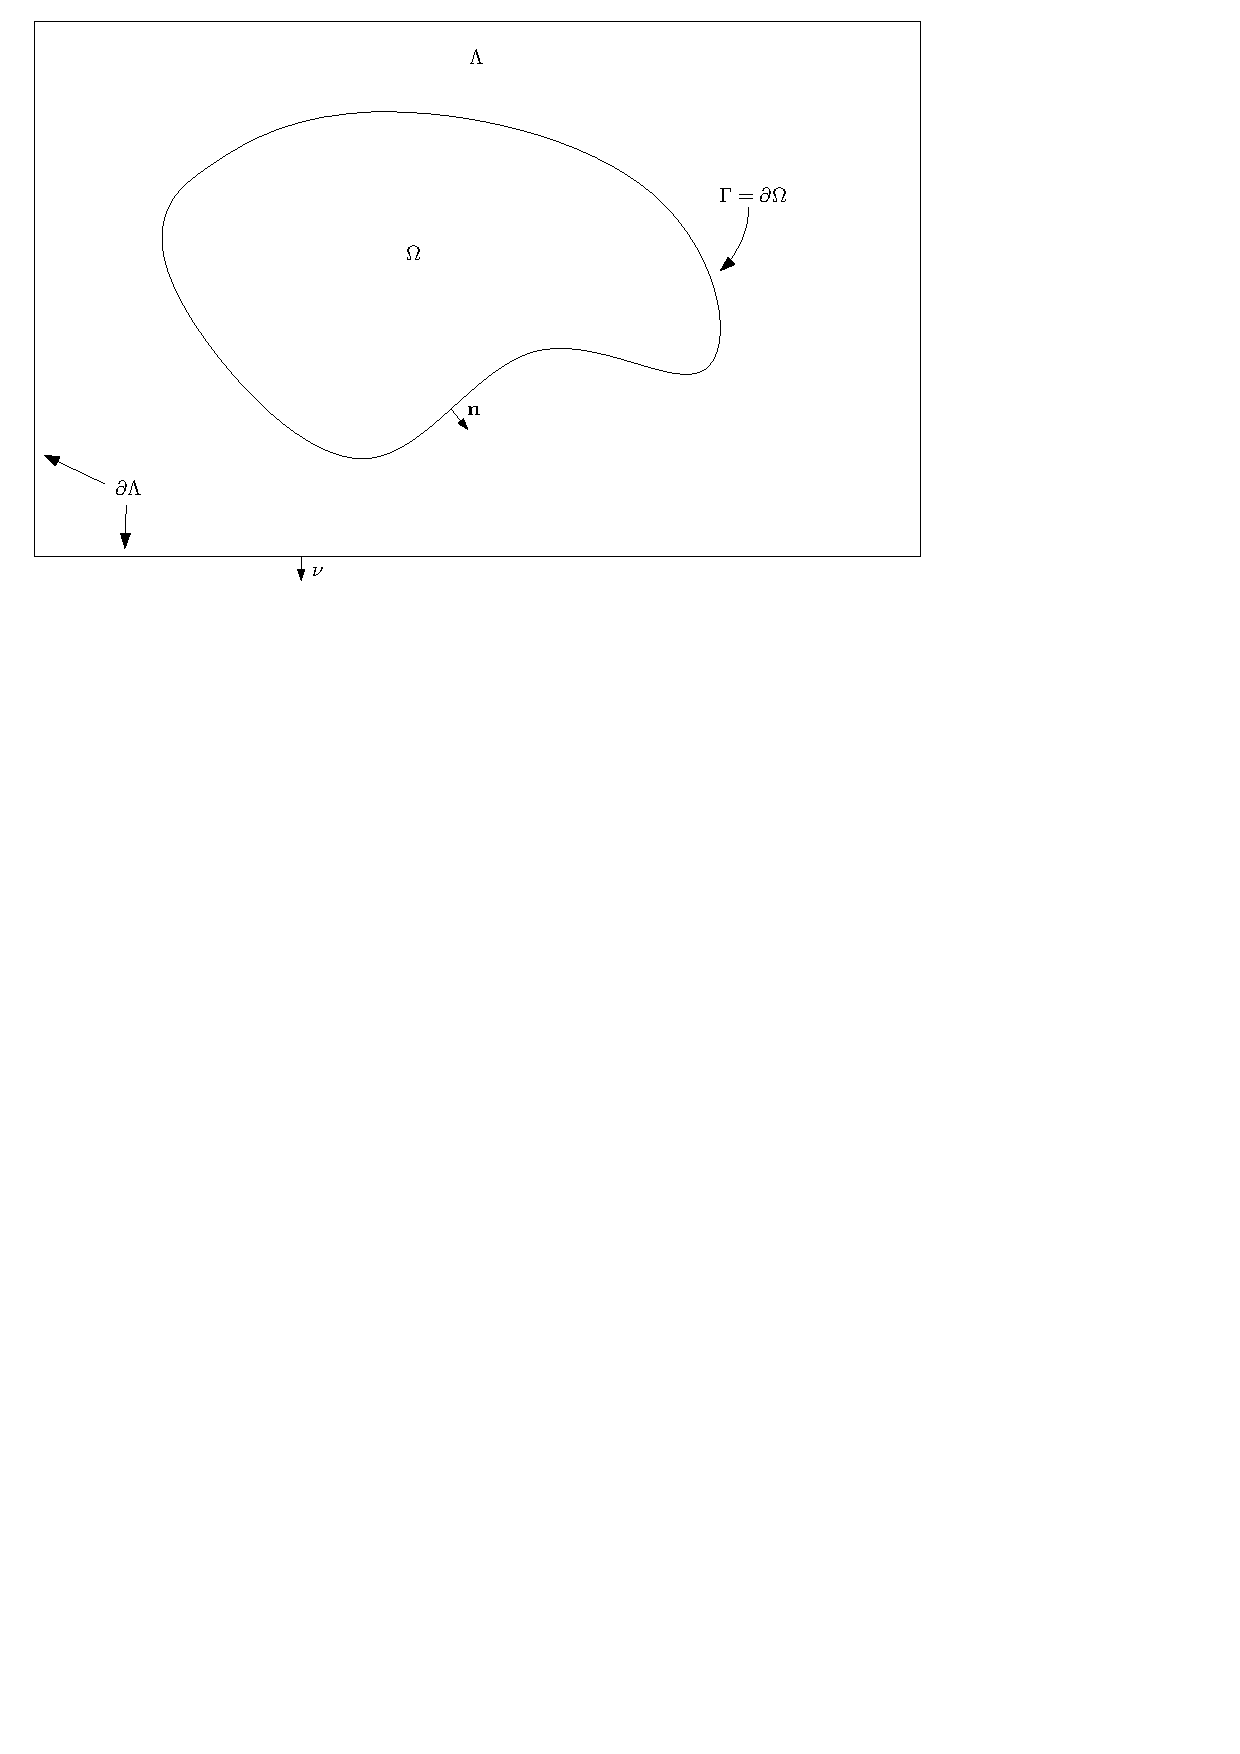
\includegraphics[width=0.65\textwidth]{DomainAndBoundaryForNavierStokes}
  \caption{Domain and Boundary with outer unit normals}
  \label{fig:DomainAndBoundary}
\end{figure}

We wish to find the velocity, $\ub\in C^{1}\left([0,T], \left[H^{2}(\Lambda)\right]^d\right)$ and pressure, $p\in C^{1}\left([0,T],H^{1}(\Lambda)\right)$ which satisfy the incompressible time-dependent Navier-Stokes equation
\begin{equation}\label{eq:nspde01}
  \begin{cases}
		\rho\left(\pf{\ub}{t} + \left(\ub\cdot\nabla\right)\ub  \right) - \nabla\cdot \sigma = \fb & \mbox{in }[0,T]\times\Lambda\\
		\nabla\cdot \ub = 0 & \mbox{in }[0,T]\times\Lambda\\
		\left[\sigma \right]\cdot\n = \fb_{\partial\Omega}  & \mbox{on }[0,T]\times\partial\Omega \\
		\ub = \fb_d  & \x \in\partial\Lambda_{d}\\
		\sigma\cdot\nu = \fb_{\nu} & \x\in \partial\Lambda_{n}\\
		\left.\ub\right|_{t=0} = \ub_{0} & \mbox{divergence free initial velocity}\\
		\left.p\right|_{t=0} = p_0 & \mbox{initial pressure.}
	\end{cases}
\end{equation}
Here $\sigma$, the (symmetric) \textbf{stress tensor}\index{sigma, stress tensor@$\sigma$, stress tensor} is chosen to be
\begin{equation}
	 \sigma = \epsilon(\ub) - pI
\end{equation}
and the \textbf{strain rate tensor}\index{epsilon, strain rate tensor@$\epsilon(\ub)$, strain rate tensor}, $\epsilon(\ub)$, is defined using the \textbf{symmetric gradient}\index{gradient, symmetric gradient@ $\nabla^{s}$, symmetric gradient}
\begin{equation}
	\epsilon(\ub) = 2\mu \nabla^{s} \ub = 2\mu\left(\frac{\nabla\ub + \nabla\ub^{T}}{2}\right).
\end{equation}
 Simplifying, we get
\begin{equation}\label{eq:nspde02}
  \begin{cases}
		\rho\left(\pf{\ub}{t} + \left(\ub\cdot\nabla\right)\ub  \right) - 2\nabla\cdot\left(\mu \nabla^{s}\ub \right) + \nabla p = \fb & \mbox{in }[0,T]\times\Lambda\\
		\nabla\cdot \ub = 0 & \mbox{in }[0,T]\times\Lambda\\
		\left[ 2\mu\nabla^{s}\ub - p I \right]\cdot\n = \fb_{\partial\Omega}  & \mbox{on }[0,T]\times\partial\Omega \\
		\ub = \fb_d  & \x \in\partial\Lambda_{d}\\
		\left(2\mu\nabla^{s}\ub-p I\right)\cdot\nu = \fb_{\nu} & \x\in \partial\Lambda_{n}\\
		\left.\ub\right|_{t=0} = \ub_{0} & \mbox{divergence free initial velocity} \\
		\left.p\right|_{t=0} = p_0 & \mbox{initial pressure}
	\end{cases}
\end{equation}

\noindent where the \textbf{density}\index{rho, density@$\rho$, density} $\rho = \rho(\x,t)\in C^{1}\left([0,T], H^{1}(\Omega)\right)$ is possibly variable, the \textbf{(dynamic) viscosity}\index{mu, viscosity (dynamic)@$\mu$, viscosity (dynamic)}\ $\mu = \mu(\x,t)\in C\left([0,T], H^{1}(\Omega)\right)$ is also possibly variable, $\n$ is the outward pointing \textbf{unit normal}\index{n, unit normal@$\n$, normal unit vector on $\partial\Omega$} vector on $\partial\Omega$ and $\nu$ is the outward pointing \textbf{unit normal}\index{nu, unit normal@ $\nu$, normal unit vector on $\partial\Lambda$} vector on $\partial\Lambda$.  We leave the forces $\fb_{\partial\Omega}$ applied on the boundary of $\Omega$ in general form, but it could be surface tension
\begin{equation}
	 \fb_{\partial\Omega} = \sigma\vec{\kappa} 
\end{equation}
 where $\sigma$ is the surface tension coefficient and $\vec{\kappa} = \kappa\n$ is the vector total curvature.

\noindent We use the standard jump notation
\begin{equation}  
	\left[ \gb(\x) \right] = \gb(\x^{+}) - \gb(\x^{-})
\end{equation}
where $\x^{+}$ is in the direction of the normal $\n$ and $\x^{-}$ is in the opposite direction.


\section{Tracking the Boundary, $\Gamma$}\label{sec:TrackingBoundaryGamma}
As the two phase boundary $\Gamma$ is free to move around the domain, but the physics depend on where it is, we must be able to track $\Gamma$.  To this end, we implement a level set method combined with a volume of fluid solver to track $\Gamma$ and use the volume of fluid calculation to enforce mass conservation of the system.  The level set method is notorious for losing volume or mass, but when combined with a volume of fluid solver and adjusted accordingly as in \cite{kees2011conservative}, we can maintain global mass conservation.  Unfortunately, there is not yet a good method to enforce local mass conservation with the level set method.

\subsection{The Volume of Fluid Method}\label{sec:VoFMEthod}

\subsection{The Level Set Method}\label{sec:LevelSetMethod}

\subsection{The Volume Correction}\label{sec:VolumeCorrection}



%
%
%
\section{Preliminaries}\label{sec:2PPreliminaries}


%
%
%
\section{Open Boundary Conditions}\label{sec:BoundaryConditions}



%
%
%
\section{General Two Phase Flow Algorithm}\label{sec:General2PFlowAlgorithm}












\appendix


%
%
%
%
\chapter{Convergence Results for Pressure-Correction Incompressible Navier-Stokes Algorithms}\label{ch:LiteratureReview}
We give a review of the main general theorems in the literature on expected convergence rates for the various forms of the projection schemes before stating the expected convergence results for the above algorithm.  While it has not been fully proved, it appears to behave qualitatively like the algorithms for which the results have been proven and the conjectures at the end summarize what we expect.  The proofs are stated without proof although reference is given to where they come from which often includes the proof or sketches of proof.

%
%
%
\section{Constant Density Incompressible Navier Stokes}

%
%
\subsection{Algorithm in Standard Form}
The numerical solution $(\ub^k, \ut^k,p^k)$ of the constant density incompressible Navier-Stokes algorithm in standard form using BDF2 time derivative has the following error estimates hold, Theorems (3.1)-(3.5) of \cite{guermond1997resultat}.

\begin{theorem}\label{thm:guermondthm3.1}
If $\ub(t,x)\in W^{1,\infty}\left(0,T;\; H_0^1(\Lambda)^d \cap H^{\ell+1}(\Lambda)^d  \right) \cap H^2\left(0,T;\; H^1(\Lambda)^d\right)$ and $p\in W^{1,\infty}\left(0,T;\; H^{\ell}(\Lambda) \right)\cap H^2\left(0,T;\; L^2(\Lambda)\right)$, then
  \begin{equation}
    \left\| \left(\ub - \ub_h \right)_{\tau} \right\|_{\ell^{\infty}\left(L^2(\Lambda)^d\right)} + \left\| \left(\ub - \ut_h \right)_{\tau} \right\|_{\ell^{\infty}\left(L^2(\Lambda)^d\right)} \lesssim \tau + h^{\ell+1}
  \end{equation}
\end{theorem}

\begin{theorem}\label{thm:guermondthm3.2}
If $\ub(t,x)\in W^{2,\infty}\left(0,T;\; H_0^1(\Lambda)^d \cap H^{\ell+1}(\Lambda)^d  \right) \cap H^3\left(0,T;\; H^1(\Lambda)^d\right)$ and $p\in W^{2,\infty}\left(0,T;\; H^{\ell}(\Lambda) \right)\cap H^3\left(0,T;\; L^2(\Lambda)\right)$, then there exist $c_s>0$ and $h_s>0$ such that for $h\in (0,h_s]$ and $\tau \leq c_s /\left(1+|\log(h^{-1})| \right)^{1/2}$ in 2 dimensions or $\tau \leq c_s h^{1/2}$ in 3 dimensions we have
  \begin{equation}
    \left\| \left(\ub - \ut_h \right)_{\tau} \right\|_{\ell^{\infty}\left(H^1(\Lambda)^d\right)} + \left\| \left(p - p_h \right)_{\tau} \right\|_{\ell^{\infty}\left(L^2(\Lambda)\right)} \lesssim \tau + h^{\ell}
  \end{equation}
\end{theorem}

\begin{theorem}\label{thm:guermondthm3.3}
Under the regularity hypothesis of Theorem~\ref{thm:guermondthm3.1} and its restrictions on $\tau$ and $h$, the error bounds also hold
    \begin{equation}
      \left\| \left(\ub - \ub_h \right)_{\tau} \right\|_{\ell^{2}\left(L^2(\Lambda)^d\right)} + \left\| \left(\ub - \ut_h \right)_{\tau} \right\|_{\ell^{2}\left(L^2(\Lambda)^d\right)} \lesssim \tau^2 + h^{\ell+1}
    \end{equation}
\end{theorem}

If we want improved error bounds for $\ell^{\infty}\left( L^2(\Lambda)^d \right)$ norm, we must add more regularity as follows:
\begin{theorem}\label{thm:guermondthm3.4}
If $\ub(t,x)\in W^{3,\infty}\left(0,T;\; H_0^1(\Lambda)^d \cap H^{\ell+1}(\Lambda)^d  \right) \cap H^4\left(0,T;\; H^1(\Lambda)^d\right)$ and $p\in W^{2,\infty}\left(0,T;\; H^{\ell}(\Lambda) \right)\cap H^4\left(0,T;\; L^2(\Lambda)\right)$, with the restrictions on $\tau$ and $h$ of Theorem~\ref{thm:guermondthm3.1}, then
  \begin{equation}
    \left\| \left(\ub - \ub_h \right)_{\tau} \right\|_{\ell^{\infty}\left(L^2(\Lambda)^d\right)} + \left\| \left(\ub - \ut_h \right)_{\tau} \right\|_{\ell^{\infty}\left(L^2(\Lambda)^d\right)} \lesssim \tau^{7/4} + \tau^{3/4}h^{\ell} + h^{\ell+1}
  \end{equation}
\end{theorem}

The estimates on the pressure norm of Theorem~\ref{thm:guermondthm3.2} can be improved by introducing a discrete norm as follows.  Let $(v_h,q_h) \in X_h\times M_h$ and define $B_h \in \mathcal{L}(X_h,M_h)$ be the discrete divergence operator $(B_h v_h, q_h) = (v_h, B_h^T q_h) = -(\nabla\cdot v_h, q_h)$.  Then define the discrete norm for $v_h \in X_h$ as $\|v_h\|_{\mathcal{A}_h} = \sup_{w_h \in X_h} (\nabla v_h, \nabla w_h)/ \|w_h\|_{L^2(\Lambda)}$ and for $q\in L^2(\Lambda)$, let $\|q\|_{B_h, \mathcal{A}_h} = \sup_{v_h\in X_h} (q, \nabla\cdot v_h)/ \|v_h\|_{\mathcal{A}_h}$.

\begin{theorem}\label{thm:guermondthm3.5}
Under the regularity hypothesis of Theorem~\ref{thm:guermondthm3.4} and its restrictions on $\tau$ and $h$, the error bounds also hold
    \begin{equation}
      \left\| \left(p - p_h \right)_{\tau} \right\|_{\ell^{2}\left(\|\cdot\|_{B_h, \mathcal{A}_h}\right)} \lesssim \tau^{3/2} + h^{\ell}
    \end{equation}
\end{theorem}


%
%
\subsection{Algorithm in Rotational Form}

\begin{theorem}
Given that the true solution is smooth enough, the numerical solution, $(\ub^k, \ut^k, p^k)$, of the constant density incompressible Navier-Stokes algorithm using the second order approximation in time, pressure correction scheme in rotational form gives the following convergence estimates:
\begin{align*}
\left\| \left(\ub - \ub_h\right)_{\tau} \right\|_{\ell^2\left([L^2(\Lambda)]^d \right)} + \left\| \left(\ub - \ut_h\right)_{\tau} \right\|_{\ell^2\left([L^2(\Lambda)]^d \right)} &\lesssim \tau^2\\
\left\| \left(\ub - \ub_h\right)_{\tau} \right\|_{\ell^2\left([H^1(\Lambda)]^d \right)} + \left\| \left(\ub - \ut_h\right)_{\tau} \right\|_{\ell^2\left([H^1(\Lambda)]^d \right)}  &\lesssim \tau^{3/2}\\
 \left\| \left(p - p_h\right)_{\tau} \right\|_{\ell^2\left([L^2(\Lambda)]^d \right)} &\lesssim \tau^{3/2}
\end{align*}

\end{theorem}
\begin{proof}
See Theorem 4.1 of \cite{guermond2004error} for details
\end{proof}


%
%
%
\section{Variable Density Incompressible Navier Stokes}

%
%
\subsection{Algorithm in Standard Form}

\begin{theorem}\label{thm:vardensityStandardFormBDF1}
If $\rho \in W^{1,\infty}\left(0,T; \; W^{1,\infty}(\Lambda) \right)$, $\ub \in W^{1,\infty}\left(0,T;\; H^1_0(\Lambda)^d\cap H^{\ell+1}(\Lambda^d) \right)$ and $p\in W^{1,\infty}\left( H^{\ell}(\Lambda)\right)$ and there exist $\chi, \eta >0 $ such that for all $k$, $\chi \leq \min_{\x} \rho^k(\x)$ and $\sup_{\x} \rho^k(\x) \leq \eta$. Assume (to decouple the density from velocity) that we can construct a sequence $(\rho^k)_k$ from a sequence $(\ub^k)_k$ of velocities in such a way that
\begin{align}
  \|(\rho - &\rho^k)_{\tau}\|^2_{\ell^{\infty}(H^1)} + \left\| \left( \rho_t - \frac{\rho^k - \rho^{k-1}}{\tau} \right)_{\tau} \right\|^2_{\ell^{\infty}(L^2)}\\
  &\leq c(\lambda)(\tau + h^{\ell+1})^2 + \lambda \left\| \Pi_h\ub(t^k) - \ub^k  \right\|^2_{H^1} + c(\lambda)\left\|\sqrt{\rho^k} \left(\Pi_h\ub(t^k) - \ub^k\right)\right\|^2_{L^2}
  \end{align}
  where $\lambda>0$ can be chose as small as is needed. And finally, we assume that the initial approximation of data 
  \begin{equation}
    \|\rho(t^0) - \rho^0\|_{L^{\infty}} + \|\ub(t^0)-\ub^{0}\|_{L^2} + h\|\ub(t^0) - \ub^0\| + h\|p(t^0) - p^0\| \lesssim h^{\ell+1}
  \end{equation}
  holds.  Then the incremental BDF1 variable density algorithm in standard form has the following error estimates
  \begin{align}
    \left\|\left(\ub - \ub_h\right)_{\tau}\right\|_{\ell^{\infty}(L^2(\Lambda)^d)} &\lesssim \tau + h^{\ell+1}\\
    \left\|\left(\ub - \ub_h\right)_{\tau}\right\|_{\ell^{2}(H^1(\Lambda)^d)} &\lesssim \tau + h^{\ell}\\
    \left\|\left(p - p_h\right)_{\tau}\right\|_{\ell^{2}(L^2(\Lambda))} & \lesssim \tau + h^{\ell}  \mbox{  (not stated or proven but should be true)}
  \end{align}
\end{theorem}
\begin{proof}
  See proof of Theorem 4.2 of \cite{guermond2011error}.
\end{proof}

\begin{conjecture}
  Under the assumptions of Theorem~\ref{thm:vardensityStandardFormBDF1}, the BDF2 standard form algorithm with variable density has the following error estimates:
  \begin{align}
    \left\| \left(\sqrt{\rho} \ub - \sqrt{\rho_h} \ub_h \right)_{\tau} \right\|_{\ell^{\infty}(L^2(\Lambda)^d)} &\lesssim \tau^2 + h^{\ell+1}\\
    \left\| \left(\ub - \ub_h \right)_{\tau} \right\|_{\ell^2(H^1(\Lambda)^d)} &\lesssim \tau + h^{\ell}\\
    \left\|\left(p - p_h\right)_{\tau} \right\|_{\ell^{2}(L^2(\Lambda))} &\lesssim \tau + h^{\ell}  \mbox{  (not stated or proven but should be true)}
  \end{align}
\end{conjecture}

%
%
\subsection{Algorithm in Rotational Form}

\begin{conjecture}
  Under the assumptions of Theorem~\ref{thm:vardensityStandardFormBDF1}, the BDF2 rotational form algorithm with variable density has the following error estimates:
  \begin{align}
    \left\| \left(\sqrt{\rho} \ub - \sqrt{\rho_h} \ub_h \right)_{\tau} \right\|_{\ell^{\infty}(L^2(\Lambda)^d)} &\lesssim \tau^2 + h^{\ell+1}\\
    \left\| \left( \ub - \ub_h \right)_{\tau} \right\|_{\ell^2(H^1(\Lambda)^d)} &\lesssim \tau^{3/2} + h^{\ell}\\
    \left\|\left(p - p_h\right)_{\tau} \right\|_{\ell^{2}(L^2(\Lambda))} &\lesssim \tau^{3/2} + h^{\ell}  \mbox{  (not stated or proven but should be true)}
  \end{align}
\end{conjecture}

This last conjecture is more of an observation of what we expect we should observe under smooth conditions.  
\begin{conjecture}
  If $\Lambda$ is smooth, for instance a circular domain, and the exact solution is smooth, then we should see the $\ell^{\infty}(E)$ norms behaving as well as the $\ell^{2}(E)$ norms in every instance.  In many cases, we cannot give a good result for the $\ell^{\infty}$ in time norms because the theory is tricky or unclear, but we should see observe them to be as good as the $\ell^2$ in time norms.  Additionally, the general theory says that $L^{2}(\Lambda)$ norm of pressure and the $H^1(\Lambda)$ norm of velocity should have $\tau^{1/2}$ power worse rates than the $L^2(\Lambda)$ norm of velocity but in smooth domains, they are often observed to all have the higher rates.  It is only when corners appear in the domain or the exact solution has less regularity that the loss appears.  
\end{conjecture}


%
%
%
%
\chapter{Various Extensions and Proofs}

%
%
%
\section{Consistency of Rotational Scheme with Variable Viscosity }
We verify that the artificial boundary conditions imposed on pressure by the rotational fix under assumptions of constant viscosity and density still roughly hold when viscosity is no longer constant.  Mainly we will show that 
\begin{equation}
  \left.\frac{\partial p^{k+1}}{\partial \n}\right|_{\partial\Lambda} = \left.\left(f^{k+1} + \nabla\cdot\ut^{k+1}\nabla\mu - \nabla\times\left(\mu\nabla\times \ub^{k+1}  \right)  \right)\cdot \n\right|_{\partial\Lambda}
\end{equation}
which is almost a consistent pressure boundary condition.  Compare this to the imposed boundary condition when viscosity is assumed constant
\begin{equation}
  \left.\frac{\partial p^{k+1}}{\partial \n}\right|_{\partial\Lambda} = \left.\left(f^{k+1} - \mu\nabla\times\nabla\times \ub^{k+1} \right)\cdot \n\right|_{\partial\Lambda}
\end{equation}
 as discussed in \cite{guermond2004error}.  
 
 Thus we are left with the distortions from the operator splitting being manifest as the tangential velocity requirement
\begin{equation}
  \left.\ub^{k+1}\cdot\n\right|_{\partial\Lambda} = 0.
\end{equation}
and an extra penalty term manifesting in the normal pressure gradient scaled by $\nabla\cdot\ut^{k+1}$.  



%
%
\subsection{Proof of consistent boundary conditions}
The following identities on a smooth vector function $\Ab$ will be of use to us:
\begin{align}
  \nabla\times\nabla\times \Ab &= \nabla\left( \nabla\cdot \Ab\right) - \nabla^2 \Ab\label{eqn:curlcurlidentity}\\
  \nabla\times\left( \mu \nabla\times \Ab \right) &= \mu\nabla\left(\nabla\cdot \Ab\right) - \nabla\cdot\left(\mu \nabla \Ab \right)\label{eqn:curlmucurlidentity}\\
  \nabla\left( \mu \nabla\cdot \Ab\right) &= \mu\nabla\left(\nabla\cdot \Ab\right) + \left( \nabla\cdot \Ab\right)\nabla\mu\label{eqn:gradmudividentity}
\end{align}

Recall that we are approximating the solution to the continuous equations
\begin{numcases}{}
  \rho\left(\frac{\partial \ub}{\partial t}  + \ub\cdot\nabla\ub\right) - \nabla\left(\cdot\mu \nabla\ub\right) + \nabla p = \fb\label{eqn:continuousmomentumequation}\\
  \left.\ub\right|_{\partial\Lambda} = 0\label{eqn:continuousvelocitydirichletbc}\\
  \nabla\cdot\ub = 0\label{eqn:continuousdivergencevelocityequalszero}
\end{numcases}
with constant density and variable viscosity.  To proceed with the proof, we start with the initial scheme (any BDF formula for time derivative will work but we give proof in terms of BDF1)
\begin{numcases}{}
  \frac{\rho}{\tau}\left( \ut^{k+1} - \ub^{k}\right) + \rho \ut^{k}\cdot\nabla\ut^{k+1} - \nabla\cdot\left(\mu\nabla\ut^{k+1}\right) + \nabla p^{k} = \fb^{k+1},\label{eqn:initialmomentum}\\ 
  \left.\ut^{k+1}\right|_{\partial\Lambda} = 0,\\
  \frac{\rho}{\tau}\left(\ub^{k+1} - \ut^{k+1}  \right) + \nabla \psi^{k+1} = 0,\label{eqn:initialprojection} \\
  \left.\ub^{k+1}\cdot\n\right|_{\partial\Lambda} = 0,\\
  \nabla\cdot \ub^{k+1} = 0,\\
  p^{k+1} = p^{k} + \psi^{k+1} - \mu\nabla\cdot\ut^{k+1}.\label{eqn:initialpressureupdate}
\end{numcases}
By applying $\nabla\times\left(\mu\nabla\times \ \cdot\  \right)$ to both sides of (\ref{eqn:initialprojection}) we observe that
\begin{equation}\label{eqn:curlcurluequalscurlcurlutilde}
  \nabla\times\left( \mu\nabla\times \ub^{k+1}\right) =   \nabla\times\left( \mu\nabla\times \ut^{k+1}\right)
\end{equation}

So by plugging equations (\ref{eqn:initialprojection}) and (\ref{eqn:initialpressureupdate}) into (\ref{eqn:initialmomentum}) and using identities (\ref{eqn:curlmucurlidentity}) and (\ref{eqn:gradmudividentity}) (with $\Ab=\ut^{k+1}$) and applying (\ref{eqn:curlcurluequalscurlcurlutilde}), we obtain

\begin{numcases}{}
  \begin{split}\frac{\rho}{\tau}\left(\ub^{k+1} - \ub^{k}   \right) + \rho\ut^{k}\cdot\nabla\ut^{k+1} + \nabla\times\left( \mu\nabla\times\ub^{k+1}\right)&\\ 
    - \left(\nabla\cdot\ut^{k+1}\right)\nabla\mu + \nabla p^{k+1} &= \fb^{k+1},\end{split}\label{eqn:momentumcwithurlculequation}\\
  \left.\ut^{k+1}\right|_{\partial\Lambda} = 0,\label{eqn:utildeonboundaryequalszero}\\
  \left.\ub^{k+1}\cdot\n\right|_{\partial\Lambda} = 0,\label{eqn:tangentialuonboundaryequalszero}\\
  \nabla\cdot\ub^{k+1} = 0.\label{eqn:divuequalszero}
\end{numcases}
By dotting (\ref{eqn:momentumcwithurlculequation}) with $\n$ and restricting to boundary and using properties (\ref{eqn:utildeonboundaryequalszero}) and (\ref{eqn:tangentialuonboundaryequalszero}), we get the normal pressure gradient condition

\begin{equation}
  \left.\frac{\partial p^{k+1}}{\partial \n}\right|_{\partial\Lambda} = \left.\left(f^{k+1} + \nabla\cdot\ut^{k+1}\nabla\mu - \nabla\times\left(\mu\nabla\times \ub^{k+1}  \right)  \right)\cdot \n\right|_{\partial\Lambda}.
\end{equation}

Finally notice that because of (\ref{eqn:divuequalszero}) and (\ref{eqn:curlmucurlidentity}), we have 
\begin{equation}
  \nabla\times\left(\mu\nabla\times \ub^{k+1}\right) = \nabla\cdot\left(\mu\nabla\ub^{k+1}\right)
\end{equation}
so 
\begin{equation}
  \left.\frac{\partial p^{k+1}}{\partial \n}\right|_{\partial\Lambda} = \left.\left(f^{k+1} + \nabla\cdot\left(\mu\nabla\ub^{k+1}\right) \right)\cdot \n\right|_{\partial\Lambda} + \left.\nabla\cdot\ut^{k+1}\frac{\partial\mu}{\partial\n}\right|_{\partial\Lambda},
\end{equation}
which is almost consistent with the momentum equation (\ref{eqn:continuousmomentumequation}).  The inconsistency comes from the $\nabla\cdot\ut^{k+1}\frac{\partial\mu}{\partial\n}$ term which can be seen as a penalty term for the normal pressure gradient.

%
%
\subsection{Note, if we use $-\nabla\cdot(\mu\ut^{k+1})$ instead of $-\mu\nabla\cdot\ut^{k+1}$ in pressure update}
In this case, we must use the identities
\begin{equation}
    \nabla\left( \nabla\cdot\left( \mu \Ab\right) \right) = \nabla\left(\mu\nabla\cdot\Ab\right) + \nabla\left( \nabla\mu\cdot\Ab \right)
\end{equation}
and 
\begin{equation}
  \nabla\left(\Ab\cdot \Bb\right) = \left( \Ab\cdot\nabla\right)\Bb + \left( \Bb\cdot\nabla\right)\Ab + \Ab\times\left(\nabla\times\Bb\right) + \Bb\times\left(\nabla\times\Ab\right)
\end{equation}
  where $\Bb = \nabla\mu$ and $\Ab = \ut^{k+1}$ to get the extra terms of inconsistency.  We end up with the following boundary conditions
\begin{equation}
  \begin{split}\left.\frac{\partial p^{k+1}}{\partial \n}\right|_{\partial\Lambda} = &\left.\left(f^{k+1} + \nabla\cdot\left(\mu\nabla\ub^{k+1}\right) \right)\cdot \n\right|_{\partial\Lambda}\\ &+ \left.\left(\nabla\cdot\ut^{k+1}\nabla\mu  + \nabla\mu\cdot\nabla\ut^{k+1} + \nabla\mu\times\left( \nabla\times\ut^{k+1}\right) \right)\cdot\n\right|_{\partial\Lambda}. \end{split}
\end{equation}



\bibliographystyle{chicago}
\bibliography{ps.bib}
% \appendix
%\input{GWVD_COETR_Consistent_Velocity_Appendix}
%\input{GWVD_COETR_Velocity_Postprocessing_Appendix}
%input{GWVD_COETR_variational_multiscale_appendix}

\end{document}
